\documentclass[sigplan, anonymous, review]{acmart}
%\documentclass[sigconf]{acmart}

%\usepackage{cite}
\usepackage{amsmath,amssymb,amsfonts}
\usepackage{array}
\usepackage{algorithmic}
\usepackage{graphicx}
\usepackage{textcomp}
\usepackage{hyperref}
\usepackage{listings}
\usepackage{subcaption}
\usepackage{xcolor}
\usepackage{numprint}
%\usepackage{booktabs} % For formal tables
%\usepackage{balance}

\newcommand{\sn}[1]{{\color{blue}\textbf{Sarah:}~#1}}
\newcommand{\jk}[1]{{\color{violet}\textbf{Johannes:}~#1}}
\newcommand{\checkNum}[1]{{\color{orange}#1}}
\newcommand{\todo}[1]{{ \color{red} \textbf{TODO:}~#1}}

\begin{document}

\title[Architectural Change vs CI Build Outcome]{On the Relationship Between Architectural Changes and Continuous Integration Build Outcome
}

\author{Johannes K{\"a}stle}
\affiliation{%
	\institution{University of Alberta}
	\city{Edmonton}
	\country{Canada}
}
\email{kaestle@ualberta.ca}

\author{Sarah Nadi}
\affiliation{%
	\institution{University of Alberta}
	\city{Edmonton}
	\country{Canada}
}
\email{nadi@ualberta.ca}

\begin{abstract}
Continuous Integration (CI) is becoming an essential component in the software development process.
However, the time cost of a CI build may often be high, if the build is broken.~\sn{isn't the cost of a build high regardless of whether it passes or fails?} \jk{The general cost of a CI build should be low. Only the time to fix a broken build is costly.}
Therefore, identifying reasons for build failure and warning developers about these likely failures can save valuable time and cost for developers.
In this paper, we investigate if there is a relationship between architectural changes and CI build outcomes.
We form two hypotheses about the relationship: (1) architectural changes lead to higher CI build failures and (2) higher CI build failures lead to architectural changes.
To investigate these hypotheses, we design a fully automated extensible framework that analyzes the architectural changes between two consecutive versions of a software system.
We use three well-established techniques to reconstruct the projects' architecture from the source code and measure change with eight metrics. 
In addition, we analyze the build logs to investigate the point of failure during the build. 
We mine almost 50,000 builds from 159 open-source Java repositories, but find no significant correlation between architectural change and build outcome. 
To enable other researchers to replicate our negative results and to investigate additional architectural metrics, we publish our framework which can easily be extended for new research questions and metrics.
\end{abstract}

\maketitle

\section{Introduction}

Continuous integration (CI) is nowadays a common practice in software development \cite{CI-Common}. It helps finding faults earlier and therefore reduces the costs to fix them \cite{NutzenCI}. On the other hand, build failures decrease the development pace \cite{Costs-BuildFailures}. Hence, by decreasing the number broken builds, the speed of development is increased whereby costs are decreased.

There are numerous research directions for predicting CI build failures. Within the context of the MSR 2017 challenge \cite{TravisTorrent}, different approaches emerged.
Multiple researches have been using meta-data about the person who was submitting the commit \cite{ContrInvolv} or meta-data from previous commits \cite{Pred-Cascade}. The latter study has shown that cascaded tree classifiers have achieved the best results with this type of data. ~\sn{the two parts here are not on the same "level".. cascaded tree classifiers are an ML technique and you can feed them any type of features while "the person submitting the commit" is one feature that is based on the meta data of the project. I think you want to re-write this paragraph to make it clearer that the point is to say that the majority of work done on CI failures used meta-data of the project instead of source code metrics (but plz verify that this is indeed true}. \jk{is this clearer?}
In general, tree classifiers are a useful machine learning (ML) technique to predict build outcome using meta data about the current and previous commits \cite{Pred-Tree}. 
These meta-data based ML approaches alone do not have high enough accuracy.

Not only meta-data, but also source code metrics impact the build outcome \cite{FailsCorr}. The impact of source code metrics on bugs and failures was already investigates by various studies \cite{MetricsSource1, MetricsSource2}. 
because it has been shown that source code metrics impact the build outcome \cite{FailsCorr}. 
In this paper, we further investigate such source code metrics. 
Bengtsson \cite{arc-metrics} has adapted source code metrics so that they are metrics for software architecture. Therefore, they should should also impact the build outcome. 
~\sn{I think you want a better transition to the architecture focus here.. can you cite a couple of papers that look at source code metrics for CI build outcome and then also cite other papers that looked at architecture change as a source of failure then say that given that source code metrics matter in CI and previous work showed that arch. changes matter in errors, it is interesting to investigate the relationship between CI failures and architectures} \jk{this better?}
Paix\~{a}o et al. found a correlation between CI build outcomes and non-functional requirements~\sn{is it *changes* in non-functional requirements? a relationship between CI and non-functional requirements themselves doesn't really make sense} \cite{Fail-NFReq}.
For example will a build break if a timing constraint is introduced, so that the code itself is not working anymore in the necessary parameters.
\jk{now clear?}
Since non-functional requirements are often addressed by software architects \cite{NFR-Architects}, it is interesting to investigate if the software architecture influences the build results or is itself influenced by continuous integration. 
This could happen if, for example, multiple builds fail and, thus, the architecture gets changed to improve the problematic area in the source code.

To investigate the relationship between CI and software architecture, it is necessary to measure the architectural change (AC) between two builds. Architectural change has been studied by different researchers in different contexts \cite{Aramis,StructDist,Arc-MDSE,Arcade-Base} , e.g.  finding the causes \cite{AC-Causes}, checking consistency with the designed architecture \cite{ArcConf, ArcCons}, investigating the impact on the business model \cite{ArcChange-Business} or the non-changed modules of the architecture \cite{Knowledge-AC}. 

Paixao~\sn{you sometimes have the special character in this name and sometimes not.. make sure to find the right spelling and fix it} \jk{he is a different person with the same last name but different spelling, thats maybe confusing, but it is correct this way} et al. \cite{ImpactAwareness} show that most developers are not aware that their code changes actually affect the architecture of the system. When made aware of the relationship, developers tend to be more careful abut their changes and they try to improve the overall architecture of the system.
Based on such previous findings, we argue that if developers realize that any architecture changes they make influence the build outcome in CI, something that affects them on a daily basis, this would further increase their awareness about the importance of the architecture of the system.

In this work, we explore the relationship between architectural change and CI build outcome.
We analyze $159$ Java Maven software systems from the TravisTorrent dataset~\cite{TravisTorrent}. 
We extract the architectural changes in every CI build by comparing the corresponding version of the system to its predecessor.
We use eight different architecture metrics from the literature to evaluate architectural changes.  
We store those extracted architectural changes along with the outcome of the build and use this data to investigate the relation between architecture and build outcome.
We hypothesize that architectural changes are either (1) preceded or (2) followed by failing builds. 
Our intuition for the first hypothesis is that many failing builds indicate a big problem in the system, which might entail changing the architecture to solve it. 
On the other hand, our intuition for the second hypothesis is that a change in the architecture may result in unexpected consequences that would then lead to build failures.

We propose the null hypotheses:

\paragraph{$\mathbf{H_0}$:} Architectural change does not correlate with Continuous Integration build outcome. 

To automate our investigation, we develop an extensible framework that runs a toolchain which automatically downloads snapshots of a software system, reconstructs the architecture, and computes change metrics. With only a few lines of code, new extractors, reconstructors, and metric calculators can be added. 
The architecture of our framework allows us to easily reuse existing architectural extraction tools and metrics, namely HUSACCT \cite{Husacct1}, ARCADE \cite{Arcade}, and Martin's metrics \cite{martinsMetrics}.

Our analysis of almost $50,000$ commits using two different architecture reconstruction techniques shows that almost no significant correlation exists between architecture changes and CI build outcome. In total, we investigated $48$ different correlations using $32$ configurations. Based on our results, we are unable to reject the null hypothesis. Architectural change does not correlate, and therefore does not impact, with build outcome.
~\sn{should we formulate this as accepting the null hypothesis? Typically, you formulate things using the null hypothesis and if you find a correlation, you reject the null hypothesis} \jk{done}


To summarize, the main contributions of this paper are:
\begin{itemize}
\item The combination of architectural change and build outcome prediction
\item The development of an easy extensible framework for 
\begin{itemize}
	\item source code and log mining
	\item architecture reconstruction
	\item architecture metric calculation
\end{itemize}
\item comprehensive study of almost $50,000$ commits
\end{itemize}


\section{Background and Related Work}

In this section, we first give some background about the terminology we use in this paper and then discuss two categories of related work. The first is work done to investigate continuous integration practices and reasons for build failure, and the second is work related to software architecture.

\subsection{Background}
TravisCI is a continuous integration (CI) tool that is tightly integrated into GitHub. CI is the process of automatically compiling, building, and testing a software system, whenever new code is pushed to the single repository. This helps developers find bugs earlier and increase the development speed \footnote{\url{https://www.martinfowler.com/articles/continuousIntegration.html}}. 
The TravisTorrent dataset \cite{TravisTorrent} consists of over 3.5 million TravisCI build samples from over 1,300 projects, written in Java, JavaScript, and Ruby.
TravisTorrent saves over fifty features for every build, including the project name, the commit ID of the build, and the build outcome.

\textit{Software architecture} is defined as the structural or hierarchical view of the system's components and the description of the relationships \cite{arcDef}. It is usually represented as a graph of the high-level components, called \textit{modules}, of a software system which are connected through links, called \textit{dependencies}. While there is no uniform standard for describing a system's architecture, it is typically modeled using Architecture Description Languages (ADLs), such as the component diagram of the Unified Modeling Language (UML)~\cite{UML-Arch}. Of course there is a huge amount of different ADLs, like Aesop, ATL or QVT \cite{ADLs1, ADLs2}.
Since there is no single way for describing an architecture, there is also no universally accepted technique for reverse engineering the architecture of a system. The most basic way is using the package structure in the code. This assumes that the developers have thought about the architecture and translated it into packages \cite{arcPkg}. In that case, high level packages correspond to modules, and module A is dependent on module B if an element of package A is using an element that is contained in package B. 
Other approaches for reconstructing architecture are ACDC or ARC, which are introduced in the following section.

\subsection{Continuous Integration}

Because Continuous Integration is nowadays getting an established technique in software development industry, there are various different research line followed \cite{ci1, ci2, ci3, ci4}. Given the nature of our work, we mainly focus on build failure prediction.

Islam and Zibran \cite{FailsCorr} have studied the relationship between build outcome, and project and build metrics. 
They found that the size of the project, the test code~\sn{not sure what that means: test code}\jk{when I write a test, this is "test code"}, and the development branch (i.e. the branch from which the build is initiated) all do not affect the build outcome.
On the other hand, the build tool used (e.g. Maven or Ant) as well as the number of changed lines and files do have an impact on the build outcome.
The fact that the previous research found that the number of changed lines and files affects the build result suggests that investigating the relationship between architectural changes and build outcome is conclusive.~\sn{I don't like the term "is a valid idea" but can't think of something better now} \jk{I tried with "conclusive", what do you think?}

In 2006, a study by Hassan and Zhang~\cite{Pred-Tree} used decision trees to investigate the relation between build failures and the meta data of developers and the project.
They achieved an specificity rate \footnote{Specificity: Rate between true negative and all negatives}~\sn{I don't know what specificity rate is.. is this an actual term? If so, change the accuracy that I use} \jk{added a footnote} of 69\%.
In an follow-up work by Ni and Li as part of the MSR '17 challenge, the prediction accuracy was further improved by using cascading tree classifiers as well as additional information about the outcome of the previous build\cite{Pred-Cascade}. 
In that research, the prediction was only done per project, because they aim to predict the error only based on this project's specific data. In consequence, the prediction is getting more accurate as more builds are in the history.
While this is certainly useful in practice, it does not help to mitigate the reasons of failing builds on a more general (i.e. cross-project) level.

Vassallo et al. \cite{CIFailTypes} have combined open and closed source projects to study the reason for build failures. Using the different maven build stages, they documented how many builds failed in which stage. They found tremendous differences between open source projects and the systems of the analyzed company, for example do open source projects fail more often during the testing phase, while closed source projects struggle more during static analysis, deployment and release. Compilation and pre-compilation errors are responsible for around $10\%$ of build failures which is relevant for our study.
Rausch et al. \cite{FailsinCIFlow} have studied reasons for failing builds, as well. They categorized 14 types of error which commonly influence the build failure based on 14 open source projects. They identified previous failing builds to be highly correlated to build failures, that means that fails often often appear in groups. In almost all of the studied projects, compilation and dependency resolvability were issues for failing builds. Other confirmed metrics which are important for studying build failure were change complexity or failing tests.

~\sn{it seems you focused the CI-related work on build failure prediction, which is OK but you need to clearly state that. Check what other categories of CI work are there and say something like there are two directions of work on CI: x [couple of main citations] and y. Given the nature of our work, we mainly focus on y. I also sent you some references that I think should be included for build failure prediction} \jk{done}

\subsection{Architecture}
\label{sec:relwork-arch}

\sn{I quickly skimmed this section but will come back it again. I feel it can be better organized. For example, can you first discuss all extraction tools and methods and then discuss how these tools/methods were used to compare intended and implemented architectues and evolution etc? You can use subsubsections for structuring for example. I feel that right  now it is not that coherent. Can you also include a citation to Gail Murphy's reflexion models http://ieeexplore.ieee.org/abstract/document/917525/ .. while it is not specific to architecture.. I think the reflexion models help find violations of architecture or somethign like that} \todo{citation done, revamp TODO, not yet quite sure how to do it}

Software architecture is a well-researched topic in software engineering.
There are generally two directions of research in the area.
The first is related to the reconstruction of the implemented architecture from the code, while the second is related to comparing this reconstructed architecture against (a) the intended or documented architecture and (b) different versions of the system (i.e., architecture evolution).
We discuss related work from both these general directions.

Already in 2001 the Gail Murphy's reflexion models \cite{MurphyRefl} considered the gap between designed and actual architecture of a software system as a problem. For that, they developed a technique to map the reverse engineered model with the designed or expected one to visualize and measure the drift between them. These reflexion models can help find violations in the architecture and are a basis for nowadays architecture conformance checking tools. 

The ARAMIS workbench \cite{Aramis} takes the step from static reconstruction of the architecture based on method calls and inheritance to extracting the data flow during runtime to check it against the predefined structure. 
For model-driven and generative software development, the task of extracting architecture is more complex than in traditional projects, because it passes through different layers of abstraction and possibly multiple DSLs. 
Thus, the way of checking consistency must account for different layers and is abstracted with architecture description languages (ADL) \cite{ArcCons,Arc-MDSE}. 
Also using ADLs, Haitzer et al. \cite{Arc-Decision} study architectural drift and erosion. In their system, the architect can simulate multiple implementation scenarios. With the help of the ADL, the program then calculates the consequences of this change, and the architect can make an educated decision which change has the best impact on the system and its architecture. 

Caracciolo et al. \cite{ArcConf} found that the automated checking of the implemented architecture with the intended one, leads to fewer architecture violations. They extracted the architecture using classic static analysis and a dependency graph. Their system checks then for violations of the MVC pattern and reports it directly to the developer. Over the course of time, fewer violations were found compared to a control group, which shows that the developers learned how to avoid architecture violations.

Nakamura and Basili \cite{StructDist} introduced the measuring of architectural distance using kernels. For that, both architectures need to be represented as a graph structure (here OO class structure) and are then compared for similar substructures. This solves the problems with renaming and is applicable to every graph. 
Because it works on the complete class graph and not an abstracted version, i.e. the architecture, this technique is not viable for consistency checking, as the designed architecture is not represented down to the class level. 
Since the graph is compared to kernels, it is necessary to define a distance measurement for this. A similar approach is used by Garcia \cite{arcade-thesis} with the cluster coverage metric.

Tonu et al. \cite{Swag} have researched architecture stability using the SWAG kit, primarily in C and C++ projects, but also introduced support for Java.\footnote{\url{http://www.swag.uwaterloo.ca/javex/}} Using four different types of metrics, growth, change, cohesion and coupling, they try to analyze when the architecture of a software system stabilizes and then predict stability for future versions. It does so by extracting facts from the source code (or in case of Java byte code) and reconstructing the architecture. A fact can be anything, from LoC to function calls and classes. 
In both studied projects, the architecture stabilizes relatively quickly and has only small changes afterwards. Unfortunately, we cannot use this tool in our research, because we want to study the source files and not the byte code of Java projects. But we do analyze change and coupling metrics.

HUSAACT \cite{Husacct1,Husacct2} is a highly customizable architecture conformance framework for Java and C\#. Dependencies between architecture modules can be defined in multiple ways and different kinds of dependencies are possible. They argue, that a ``call'' dependency cannot be compared directly to a ``inherits'' dependency and, hence, must be treated differently. 
The framework extracts several types of dependencies between source code elements (e.g. classes, interfaces, packages). HUSAACT needs to have a module specification, i.e. which root packages or classes are part of which architecture module. If given this, it maps the defined architecture vs the real implementation and reports violations.
If no such specification is available, it is not possible to compare two versions of software on a higher level than the implementation graph. 
Hillemacher \cite{MScSteffen} has compared four different tools for architecture extraction and conformance checking and elected HUSACCT to be the best extraction tool, which is what we need here.

In his PhD thesis \cite{arcade-thesis}, Garcia developed the ARCADE framework. It is used to detect architectural decay, also called thrift and erosion, as well as architecture smells. During this, various recovery techniques were compared \cite{arcRec-comparison}, whereat ACDC \cite{ACDC} and ARC were the most successful. 
ACDC clusters modules based on patterns. Patterns are, for example, if two elements are in the same package, are used together, or if they depend on the same resources. For Java, ACDC recovers the architecture from the class files. ARC is introduced by Garcia himself, clusters entities based on semantic similarity using a statistical language model based on comments and identifiers in the source code.
The ARCADE framework uses these different recovery techniques to compute similarity metrics, namely a2a (architecture to architecture) and cvg (cluster coverage) \cite{Arcade}. 
The first one defines similarity based on the minimum number of steps to get from one architecture graph to the other. For example, removing one dependency or adding one node is each one step. While a2a looks at the architecture from a top-level perspective, cvg looks into the modules, or clusters, and computes if they are still the same module. For example, if all classes in a module are changed but the module name itself is untouched, it cannot still be considered to be the same module. Hence, it compares the entities inside the modules and only considers two modules equal, if at least $x \%$ of the entities are equal.

One reason for failing builds are syntax errors. Because builds with syntax errors are uncompilable, we do not want to use recovery techniques which rely on the compiled class files. Thus, we do not use the SWAG Kit or ARCADE directly.
However, the metrics and the recovery technique are promising in our context. Hence, we combine the strengths of HUSAACT in extracting the structure from the source files with the recovery technique ACDC and the metrics from ARCADE. 
In previous studies, other researchers \cite{MScSteffen, arcRec-comparison} have given us confidence that the choices HUSACCT and ACDC are indeed some of the best tools, which we can use.
The cvg metric is comparable to kernel based similarity whereas a2a considers change. Coupling in the architecture will be addressed with Martin's metrics. We reuse the modules from HUSACCT and ARCADE directly, while we need to implement the Martin's metrics ourself. 

\section{Architecture Metrics Used} \label{sec:Metrics}

As part of our work, we need to extract metrics that describe the architectural change that happened in a given version of the code. 
In Section~\ref{sec:relwork-arch}, we provided a general description of several approaches that exist in the literature.
In this section, we provide a detailed description of the eight \jk{yes, 8 is right, we could refer to table 2 here.} metrics we use in our work, and the reasoning behind the choice.


\paragraph{Martin's metrics} 
The first set of metrics we use have been developed by Robert Martin~\cite{martinsMetrics}.
We refer to the set of metrics he introduced as \textit{Martin's metrics}.
Specifically, we use three of the five metrics: \textit{afferent} coupling (Aff), \textit{efferent} coupling (Eff), and instability (I).
These metrics describe the independence of modules. 
\textit{Coupling} describes how many incoming (i.e., afferent) or outgoing (i.e., efferent) transitions a module has. 
For example, if class \texttt{Car} of module \texttt{Vehicles} implements the interface \texttt{Engine} of the module \texttt{Parts}, then \texttt{Vehicles} has an outgoing transition to \texttt{Parts}, and \texttt{Parts} has the corresponding incoming transition. 
In other words, \texttt{Vehicles} depends on \texttt{Parts}.
\textit{Instability}, shown in Equation~\ref{eq:inst}, is then defined as the ratio between efferent coupling and the complete coupling.
The equation shows if a module is highly dependent on other modules ($I$ close to 1) or if many modules depend on it ($I$ close to 0).

\begin{equation} \label{eq:inst}
I = \textit{Eff} / (\textit{Eff} + \textit{Aff})
\end{equation}

In the context of architectural change, the instability metric can be used as follows. If the instability of a given module changes, then this module must have had an increase or decrease in its number of dependencies. 
Obviously, a corner case is if the module had the exact same number of changes in its afferent and efferent coupling, leading to a constant instability value despite the changes.

\paragraph{\textit{a2a} and \textit{cvg}} More sophisticated change metrics are Architecture to Architecture {a2a} and Cluster Average (cvg). 

a2a measures the minimum amount of steps to get from the first to the second architecture divided by the sum of the steps needed to build both architectures themselves (Equation \ref{eq:a2a}). A step is either the adding, removing, or moving of an entity inside a module or the creation or deletion of a module. 

\begin{gather} \label{eq:a2a}
a2a(A_i, A_j) = 1 - \frac{mto(A_i, A_j)}{aco(A_i) + aco(A_j)}
\intertext{where:}
\begin{tabular}{>{$}r<{$}@{\ =\ }l}
mto(A_i, A_j) & steps from $A_i$ to $A_j$ \\
aco(A_i) & steps to create $A_i$
\end{tabular}\nonumber
\end{gather}


cvg is a metric that measures how a given module is changing. For that, the \textit{Cluster to Cluster} (c2c) metric is calculated, which defines how many elements of the cluster overlap divided by the number of elements in the bigger cluster (Equation \ref{eq:c2c}) In the context of architecture a cluster is synonymous to a module.
As an example, if a module has 20 elements, and from one version to another, two elements get removed and three are added, then $c2c = \frac{18}{21}$. 
If this ratio is above a predefined threshold $th_{cvg}$, the clusters are considered similar, according to the similarity metric $simC$ in Equation \ref{eq:simC}. The cvg metric then calculates the ratio between equal modules and the amount of modules in the architecture (Equation \ref{eq:cvg}). In ARCADE \cite{Arcade}, the cvg is calculated with a threshold of $75\%$ from the earlier version to the latter one ($\text{cvg}_\text{src}$) and with $66\%$ the other way around ($\text{cvg}_\text{tar}$). These are the standard settings in ARCADE, but it is not explained why these numbers are chosen. One explanation might be that adding functionality to a module does not change its behavior as much as removing elements. Therefore, the higher threshold for $\text{cvg}_\text{src}$ is accounting for this.~\sn{this is confusing.. is this assuming that the next version always adds and not removes?} \jk{its more, if I got from 3 to 4 it's 33\% change, but if I go from 4 to 3 it's only 25\% change.}

\begin{equation} \label{eq:c2c}
c2c(c_i, c_j) = \frac{|\text{entities}(c_i) \cap \text{entities}(c_j)|}{\max(|\text{entities}(c_i)|, |\text{entities}(c_j)|)}
\end{equation}

\begin{equation} \label{eq:simC}
\begin{split}
simC(A_i, A_j) = \{c_i | c_i \in A_i, \exists c_j \in A_j) \\ 
(c2c(c_i, c_j) > th_{cvg})\}
\end{split}
\end{equation}

\begin{equation} \label{eq:cvg}
cvg(A_i, A_j) = \frac{|simC(A_i, A_j)|}{|allC(A_i)|}
\end{equation}

\paragraph{Combining metrics} 
~\sn{I don't really understand how you combine them. Can you elaborate?} \jk{Maybe combine is just the wrong word. I mean I just use all of them as a set. }
The problem with a2a and cvg is that they do not explicitly take the dependencies between modules into account. This is only done while reconstructing the architecture itself, which we do with the pattern based ACDC from the ARCADE framework. 
To get a view of the change of the dependencies explicitly, we combine a2a and cvg with the widely accepted Martin's metrics \cite{Val-MartinsMet}, which especially account for the change in between the modules. 

\section{Methodology for Architectural Comparison}

\begin{figure*}[!t]
	\centering
	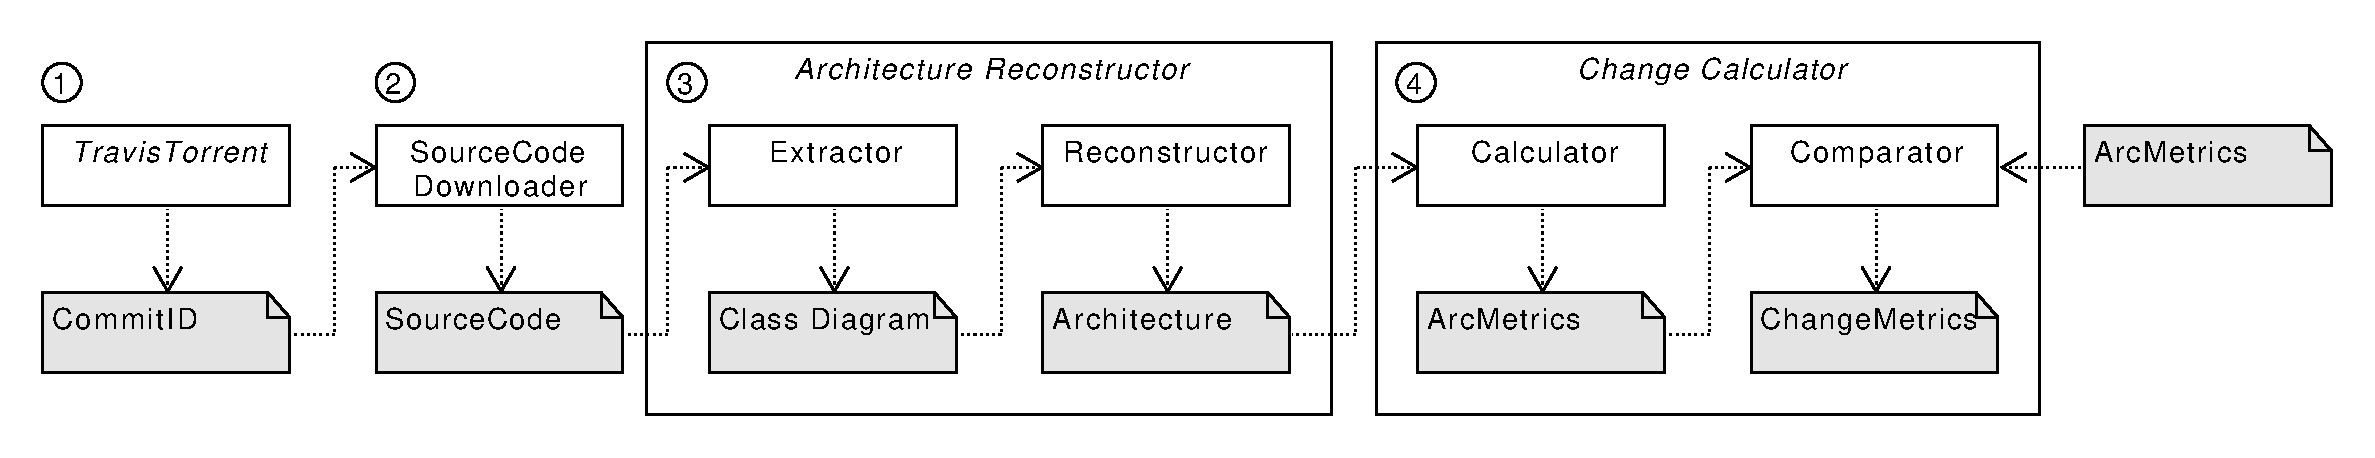
\includegraphics[width=7in]{assets/combined.pdf}
	\caption{Process from Dataset to Change Metrics \jk{Is this figure better?}}
	\label{architecture}
\end{figure*}

\begin{table}
	\caption{Ten Largest Projects under Study}
	\label{tableProjects}
	\centering
	\scalebox{0.9}{
	\begin{tabular}{ | c | c | c | c | c | }
		\hline
		project name & commits & analyzed & range & project type \\
		\hline
		sonarqube & 11590 & 4573 & 1.25y & Code Analyzer \\
		graylog2-server & 8490 & 842 & 4.25y & Log Analyzer \\
		okhttp & 5367 & 1770 & 3.5y & HTTP Client \\
		cloudify & 4984 & 821 & 2.5y & Dev. Framework \\
		structr & 3809 & 1253 & 2.5y & Development App \\
		owlapi & 3238 & 2178 & 3.5y & OWL API \\
		jOOQ & 3196 & 451 & 3y & SQL API \\
		checkstyle & 3029 & 325 & 2y & Code Analyzer \\
		vectorz & 3025 & 46 & 3.5y & Math Library \\
		owner & 2671 & 2099 & 3.5y & Property Files API \\
		\hline
	\end{tabular}
	}
\end{table}


To establish the relationship between architectural changes and CI build outcome, we need to determine the architectural changes that occurred between two versions of the system.
In this section, we describe the methodology we use to calculate these architectural changes.
Figure \ref{architecture} shows an overview of the methodology we use.
We first read the commit ID of the build out of the TravisTorrent dataset and then download the source code to this commit. Inside the architecture reconstruction, we first extract the class diagram to then reconstruct an architecture based on the classes. 
The extracted architecture is used to calculate metrics based on this architecture and these metrics are then compared with the architecture metrics from another commit to compute a set of architectural change metrics.
The complete source code of the framework, as well as our results which are explained later, can be found online\footnote{\url{https://github.com/jodokae/cmput663-architecture}. Note that this is an anonymized GitHub repo to comply with the double blind policy.~\sn{make sure to change the URL}} \todo{URL change}
 
\paragraph{Step 1} extracts the unique commit ID of each CI build from the TravisTorrent database.

\paragraph{Step 2} uses the commit ID extracted in step 1 to download a snapshot of the project from GitHub.


\paragraph{Step 3} extracts the architecture information needed to compare two commits in the next step. 
Specifically, Step 3 is split into two parts, (a) the extraction of the class structure and (b) the reconstruction of the architecture. 

In Step 3a, we use the extractor of the HUSACCT framework \cite{Husacct1} to extract relation triples in the form of relationship type, source, target (see listing \ref{lst1:rsf}), and save this information in the Rigi Standard Format (rsf) \cite{RSF}, because the ARCADE tools rely on this format. This relational system is easy convertible into a graph structure or a database and stores the modules implicitly in the dependencies. 
~\sn{I don't understand the next part about the downside. please elaborate} The downside of this format is that the modules cannot be extracted separately but only implicitly while analyzing the dependencies. That is compareable to the absence of a \texttt{getVertices()} method, and you need to traverse all dependencies to get a full list of the nodes. \jk{does this help?}
Fortunately, this is irrelevant for our work. For simplicity the dependency types are restricted to ``subPkg'', ``contains'' and ``references'', where ``subPkg'' means that a package is a sub package of another one, ``contains'' means that that a package contains a Java type, and ``references'' is any dependency between two Java types. The results are then fed into the reconstruction.

\begin{figure}[!t]
	\centering
	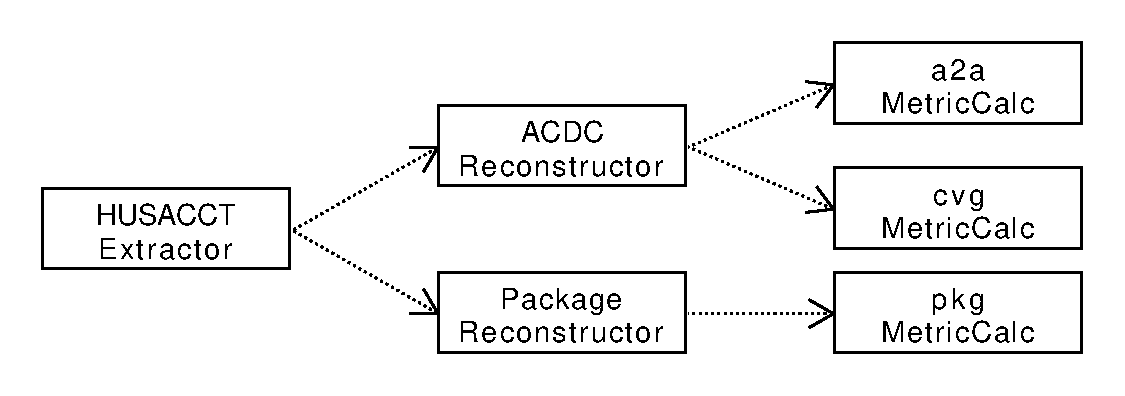
\includegraphics[width=3.45in]{assets/implementedArc.pdf}
	\caption{Implemented tool chain}
	\label{implToolchain}
\end{figure}

\begin{lstlisting}[
frame = single, 
belowskip=-0.8 \baselineskip,
float,
caption=Rigi Standard Format example,
label=lst1:rsf,
columns=flexible
]
subPkg   checkstyle checkstyle.grammars
subPkg   checkstyle checkstyle.gui
contains checkstyle checkstyle.Main
references checkstyle.Factory checkstyle.Main
\end{lstlisting}

\begin{table*}
	\caption{Metrics}
	\label{tableMetric}
	\centering
	\begin{tabular}{ | c | l | l | c |  }
		\hline
		Name & Full Name & Description & Builds With Change \\
		\hline
		\#V & Number of Vertexes & Number of changing modules & 1.6\%  \\
		\#E & Number of Edges & Number of changing dependencies & 3.6\% \\
		A. Inst & Absolute Instability & Change of instability for weighted dependencies & 16\% \\
		R. Inst & Relative Instability & Change of instability for unweighted dependencies & 3.4\% \\
		deg & Average node degree & Sum of Edges (unweighted) per module & 3.1\% \\
		a2a & architecture to architecture & number of steps to get from one architecture to another & 67\% \\
		$\text{cvg}_\text{src}$ & cluster coverage (source) & \% of changed modules based on the earlier arch & 39\% \\
		$\text{cvg}_\text{tar}$ & cluster coverage (target) & \% of changed modules based on the latter arch & 40\% \\
		\hline
	\end{tabular}
\end{table*}


In Step 3b, we reconstruct the architecture of the current version of the system based on the information extracted in Step 3a. We use two different architecture reconstruction techniques.

The first is ACDC, because it has one of the best reconstruction accuracy rates when compared to other commonly used techniques \cite{arcRec-comparison}. 
While an implementation of ACDC is provided in the ARCADE framework, this implementation works directly on the Java byte code.  Given that a common reason for failing builds (in our work $10\%$ of the builds, $11\%$ in Vassallo et. al \cite{CIFailTypes}) is compilation errors, it is thus better if we can instead use directly the source code for extracting the architecture. This is why we have Step 3a where we extract the class structure using the source-based HUSACCT extractor, and then feed that information into ACDC after deactivating its own first level extraction.~\sn{you don't really re-implement it then.. it is just a minor modification right?}\jk{right, I changed it to use there}

The second reconstruction technique is package reconstruction, which is often used as ground truth analysis \cite{arcRec-comparison}. 
\sn{ why do we need two techniques ?} \jk{we use 2, because I found the ACDC architecture confusing to use. And when we have two, we can claim, that its not the fault of the recovery technique, that we didn't find anything} 
We implemented this techniques ourselves based on the HUSACCT extraction.
This technique looks for the root packages in the system. If there are only a few root packages, it is assumed that the implemented architecture lies a level deeper in the packages. For example, if there is only the ``org.sonar'' as root, this is just the base container and not an architectural element. Therefore, all direct children of this package are considered as modules until there are at least an acceptable number of modules. In this work, we consider 10 as the minimum amount of modules needed. This number was chosen with manual sampling over different projects, so that the achieved results were the most consistent with the believed~\sn{believed? by who?}\jk{by me ... I needed to define a value, so I tried to find one, which gave results that seemed to be components} intended architecture. We follow Song et al.'s approach of considering all ``references'' edges as dependencies~\cite{ArcAsGraph}. 

\paragraph{Step 4} calculates the architectural changes between two given commits.
As explained in Section \ref{sec:Metrics}, we use the ARCADE metrics a2a and cvg as well as Martin's metrics. We calculate the ARCADE metrics on the architecture extracted by ACDC. Cvg is calculated twice, one based on the modules of the first version (called \textit{source}) and one based on the second version (called \textit{target}).
The coupling metrics are calculated on the package architecture to have some ground truth metrics for comparison. We calculate five package metrics, some basic information on the package based architecture and the Martin's metrics; thus, we have 8 metrics in total summarized in Table \ref{tableMetric}.
For every module, the absolute number of incoming and outgoing edges are calculated, the degree of the node (sum over ingoing and outgoing edges), as well as the absolute and relative instability. The absolute instability is based on the absolute number of connections between the modules, i.e. if Module A has only three ingoing connections from Module B, then the afferent coupling is considered three. For the relative instability, the coupling is booleanized, i.e. is $0$ if there is no connection or $1$ if there is one, so it is not measured how tightly connected two modules are, just if they are connected at all.
Since we need to calculate the change for the complete architecture, and not for each module, we calculate the mean instabilities and node degree as well as the absolute number of modules (vertexes) and dependencies (edges).

We then perform a pairwise comparison of each metric. To compare proportional metrics, like instability, the difference between the values is taken, e. g. if architecture A has an average instability of $30\%$, and architecture B has an average instability of $25\%$, then they are $5\%$ different to each other (Equation \ref{eq:relDiff}. For metrics with absolute numbers, like node degree, we calculate the similarity as the proportion of the two values, e.g. A has an average node degree of $8$ and B has $10$, then they are $80\%$ similar, i.e. $20\%$ change (Equation \ref{eq:absDiff}).

\begin{equation} \label{eq:relDiff}
c_{rel}(m_1, m_2) =  \max\{m1, m2\} - \min\{m1, m2\}
\end{equation} 

\begin{equation} \label{eq:absDiff}
	c_{abs}(m_1, m_2) = 1 - \frac{\min\{m1, m2\}}{\max\{m1, m2\}}
\end{equation} 


We save the corresponding comparison results of each pair of architectures, corresponding to two consecutive commits, in a JSON file. Given the architecture of our framework, our methodology can easily be expanded with more architecture reconstructors or metric calculators. 

~\sn{the rest of this paragraph is not clear.. and I wonder if it should be moved somewhere else} \jk{reformulated}
To add another module to the framework, one needs only to implement a new subclass for the changing module, store its result in the Rigi Standard Format and it can be integrated with all existing tools. 
In this way, we have combined HUSACCT and ACDC and integrated it with the ARCADE metrics. Similarly, we have implemented the package reconstruction and metrics, so that both ways of computing change can be run independent or simultaneous (Fig. \ref{implToolchain}).

\jk{this paragraph has to be in section AC, not CI build}
Because the build tool impacts the outcome of the build but not the architecture itself \cite{FailsCorr}, we limit the study to only one build tool. Although this introduces bias, it ensures consistent results in return. HUSACCT needs the path to the source files, so we can exclude test files and resources. Therefore, we choose the build tool maven with its convention over configuration paradigm. In this way we can be sure where everything is stored in the file structure. This eases the implementation of the class structure extraction. ~\sn{don't understand the next part} \jk{clearer now?}
Some commits get built more than once. Because it is impossible that the architecture changes between these builds, we only consider one of them. 
We haven chosen the first build which uses this commit, because the following builds change most likely only the configuration of the CI server. 
Thus, we can ensure that changing configuration does not bias the results. Instead, we compare the changing source code based on the older configuration, i.e. the configuration which is equal to the one of the older build. 

\section{Methodology for CI Build Outcome Extraction}
\label{sec:ci-build-outcome}

\jk{Is this better?}
The extracted architecture change metrics are compared and correlated to software faults. In this study, we use the CI build outcome as a metric for faults. 
As Vassallo et al. \cite{CIFailTypes} described, there are different type of failures in a build. They classify based on the Maven goals. Given that we already introduced compilation errors as one possible source for failing builds, this is a sound approach. Because we cannot run every maven goal separately for every build we analyze, since it is too costly, we use a simpler approach. 
Furthermore, because some builds are already older and have dependencies which are not anymore available or need to be installed manually, the approach to rerun everything may even be impossible. Still, we base our heuristic on the Maven goals.
Hence, we analyze the log files from TravisCI for all builds, to classify the build outcome further, than in success and failure. We used a heuristic to filter first lines that start with the ``\texttt{[Error]}'' keyword, which is used by the Maven log to indicate defects. Afterwards, we look for ``Compilation failure'', ``dependencies'' or ``test failures'' to categorize the failures. We map this with the actual build result to mitigate errors in the heuristic, so that only if the actual build failed, we use one the fail categories. We end up with five possible build results: (0) no error, (1) error during dependency resolution, (2) compilation failure, (3) test failure or (4) unknown error. 

\section{Evaluation Setup}

We now explain the setup we use for our evaluation.

\paragraph{Data Set.}
To investigate our hypotheses, we analyze projects from the TravisTorrent dataset, which use Java and Maven. 
The TavisTorrent dataset contains $241$ projects that use Java as their main programming language and are built with Maven. 
From these $241$ projects, we exclude ones that have have less than two commits on the master branch, because we need at least two commits to be able to compare architectures. 
This left us with \todo{$X$} projects.
We further filter this list to exclude projects where we could not retrieve their builds or logs from GitHub and TravisCI~\sn{why would this ever happen? aren't these stored in the travistorrent data set?} \jk{no, only the IDs which link to the server, but some are just not present anymore}, or where our toolchain was unable to reconstruct the architecture~\sn{again why would this happen?} \jk{bugs, download errors .. various reasons, some are problems in the code, others problems with the used tools.. and some I just don't know. That's why I just gave the beginning and the end number, because we lost here the most projects. But I don't think it would change the results.}
This left us with $159$ projects to analyze, containing a total of
$49,531$ commits. A list of the ten biggest analyzed projects, in terms of total number of commits~\sn{what is an unrestricted commit?}\jk{bad wording, total number of commits and not number of commits after our restrictions took place}, can be found in table \ref{tableProjects}.

The pass rate of the studied projects is $84.9\%$. Around $10\%$ of the builds failed because of errors before or during the compilation of the software. One third of the errors could be mapped to test errors. We did not further separate the other types of failures, but sampling shows that some of the reasons for the other category include configuration errors or incorrect maven plugins.
The active time of the projects in the data set varies.
For the ten biggest projects (in terms of number of commits), it is between one and four years of development time, some of which start at a well-established state (the TravisTorrent dataset starts, for example, at build number 500 for SonarQube), while others start at build 1 (e.g. Checkstyle)~\sn{ is the part about where they start general to all projects or to the top 10?} \jk{does it matter? If it's true for 10, it is also true for all.}.
The projects also belong to a range of different domains.
In the ten biggest projects, there are two code analyzers, three APIs~\sn{libraries? and what kind of libraries? libraries have domains too} \jk{c.f. table 1. I thought it sounds better to say three APIs then, one x API, one y API and one z API. And I used the self description of the projects for this, if they classified themself as API, then I said it's an API}, a web client and an IDE, some for databases, linear algebra or ontologies. Table \ref{tableProjects} gives a detailed list.


\paragraph{Calculated Correlations.}

The calculated architectural metrics are tested for correlation with the build result. This is done in multiple ways. First, the metric is tested against the direct build outcome, then the previous or following $b$ outcomes for $b \in \{2, 3, 5, 10\}$. This means that we look for correlations between a change in build $x$ and the build result in builds $\{x, x \pm 1, \hdots, x \pm b\}$. From this, we can see if architectural change correlates to build failures in recent history or near future (i.e., the relationships mentioned in our hypothesis). 
~\sn{Before I try to rewrite this, I need to  understand why you don't consider the individual types of build failures if you differentiate between them? So if you do record why the build failed, why don't you see if there is a correlation with failure in general and then with the individual types of failure?}\jk{I consider the type of failure in the direct correlations with the corresponding build. If I do it with multiple builds, then I have to correlate AC: x \% with the next n Builds: [0, 1, 2, 2, 0], which would be 0 succ builds, 1 error type A, 2 error type B, 2 error type C etc. And I didnt' had a idea how to measure this type of correlation. Then i simplified it to "in the next 5 builds, there are 2 failures".} Because there are different reasons for a CI build failure (see Section~\ref{sec:ci-build-outcome}), for testing in the near past and future, the fail types get categorized into non-failure and failure. In this way, we get a single integer of how many builds failed, instead of having multiple variables. 
Then, for every architectural metric, the change gets classified from its continuous value into the two categories 'change' and 'no-change'. For that, we consider a threshold $t \in \{0.01, 0.02, 0.03, 0.04, 0.05, 0.1, 0.2, 0.5\}$, where every change above this threshold is considered a change, and everything below as no change. 
We chose this range of thresholds, because most of the architectural changes in our dataset were small (Figure \ref{fig:histograms}). 
We take different thresholds at all to figure out if small changes affect the measured correlation. 
For every calculated comparison that includes no Boolean variables, the correlation test is run with Pearson's test, while others are run with Spearman's test. ~\sn{this previous paragraph generally needs another revision} \jk{better?}

\begin{figure*}[!t]
	\centering
	\begin{subfigure}{2.3in}
		\centering
		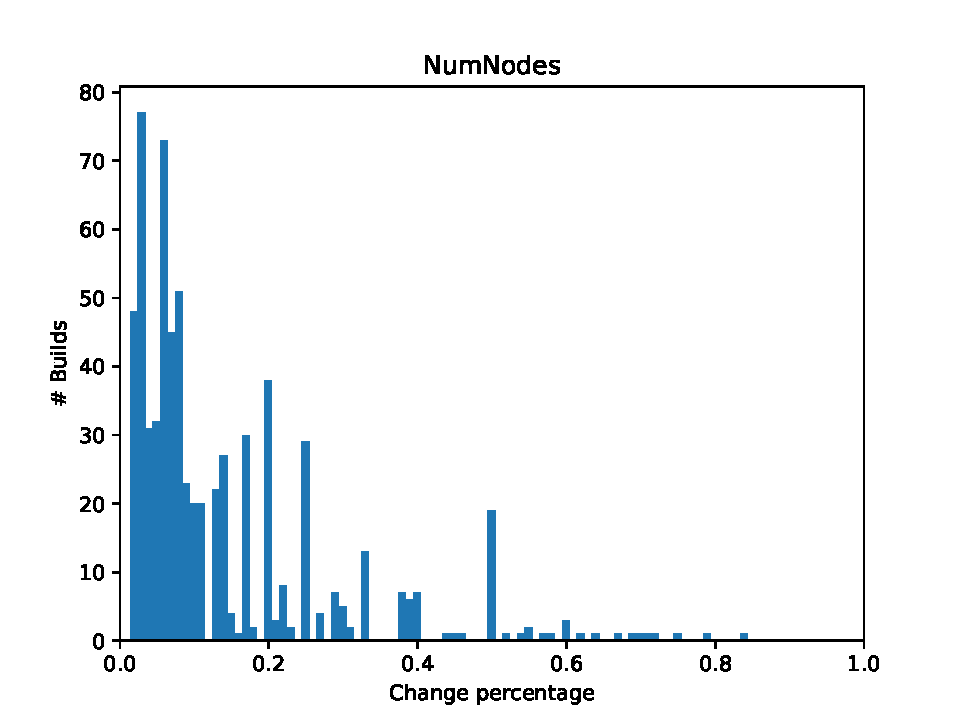
\includegraphics[width=2.3in]{assets/NumNodes.pdf}
		\caption{\#V}
		\label{numNodesHist}
	\end{subfigure}%
	\begin{subfigure}{2.3in}
		\centering
		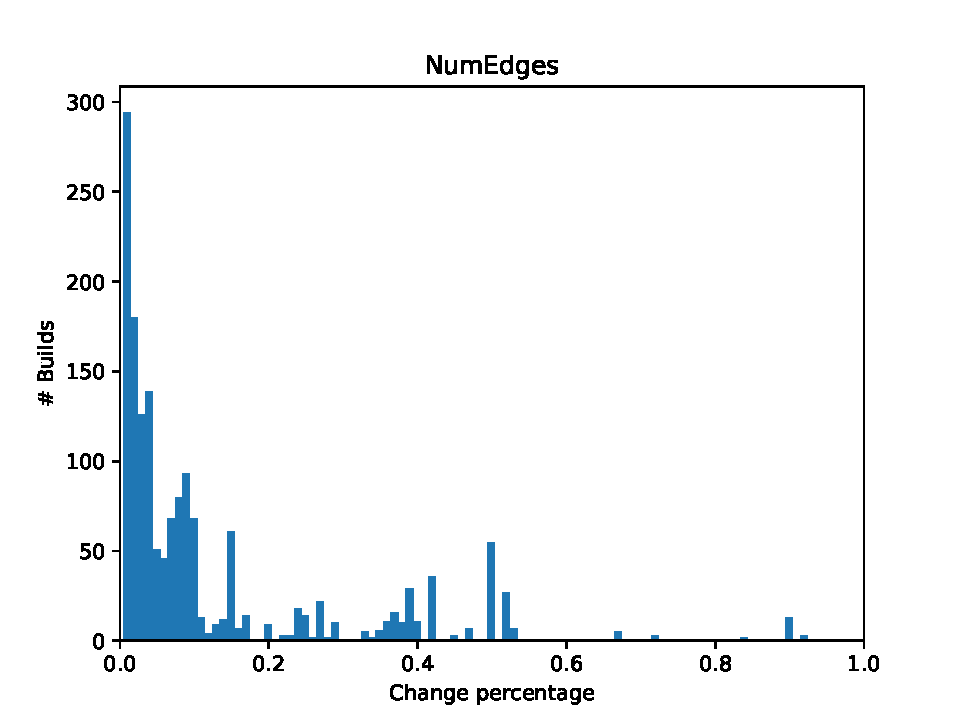
\includegraphics[width=2.3in]{assets/NumEdges.pdf}
		\caption{\#E}
		\label{numEdgesHist}
	\end{subfigure}%
	\begin{subfigure}{2.3in}
		\centering
		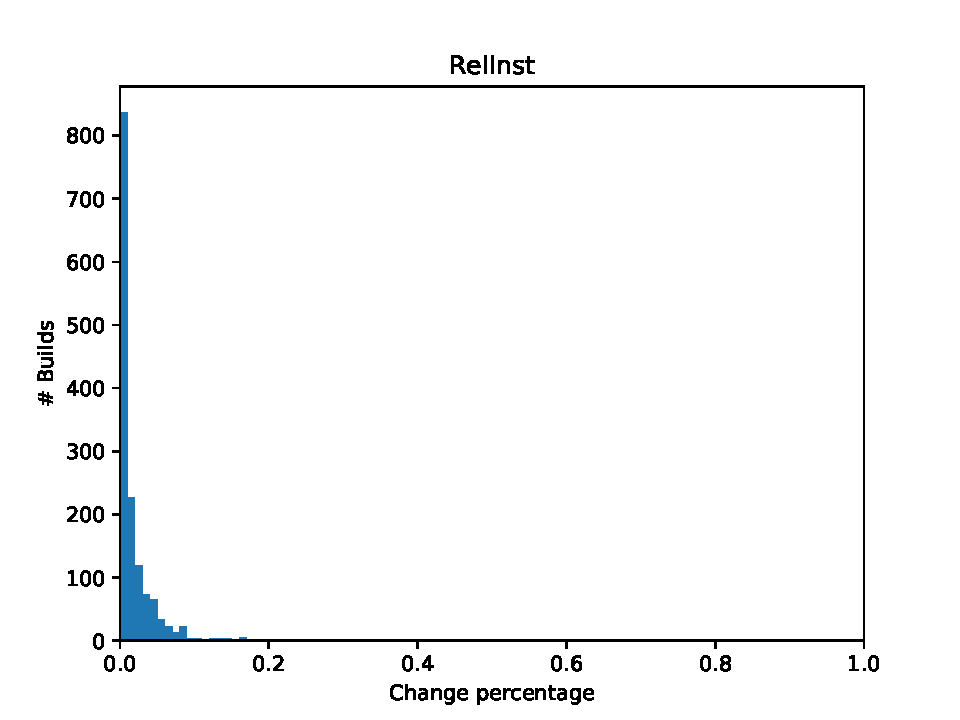
\includegraphics[width=2.3in]{assets/RelInst.pdf}
		\caption{rel. Inst}
		\label{relInstHist}
	\end{subfigure}
	\begin{subfigure}{2.3in}
		\centering
		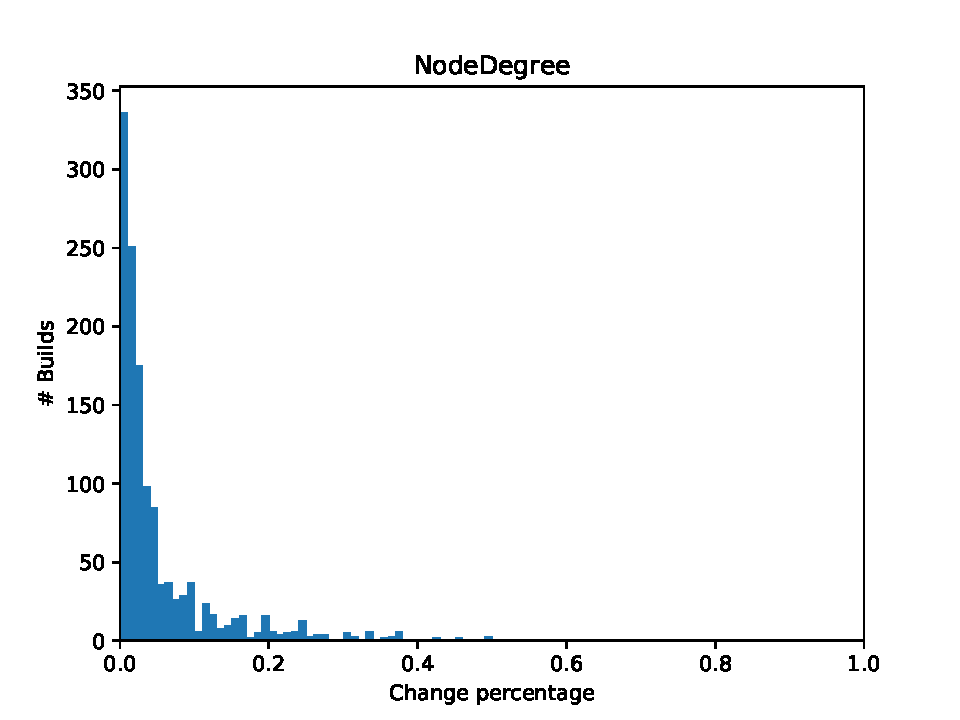
\includegraphics[width=2.3in]{assets/NodeDegree.pdf}
		\caption{deg(V)}
		\label{nodDegHist}
	\end{subfigure}%
	\begin{subfigure}{2.3in}
		\centering
		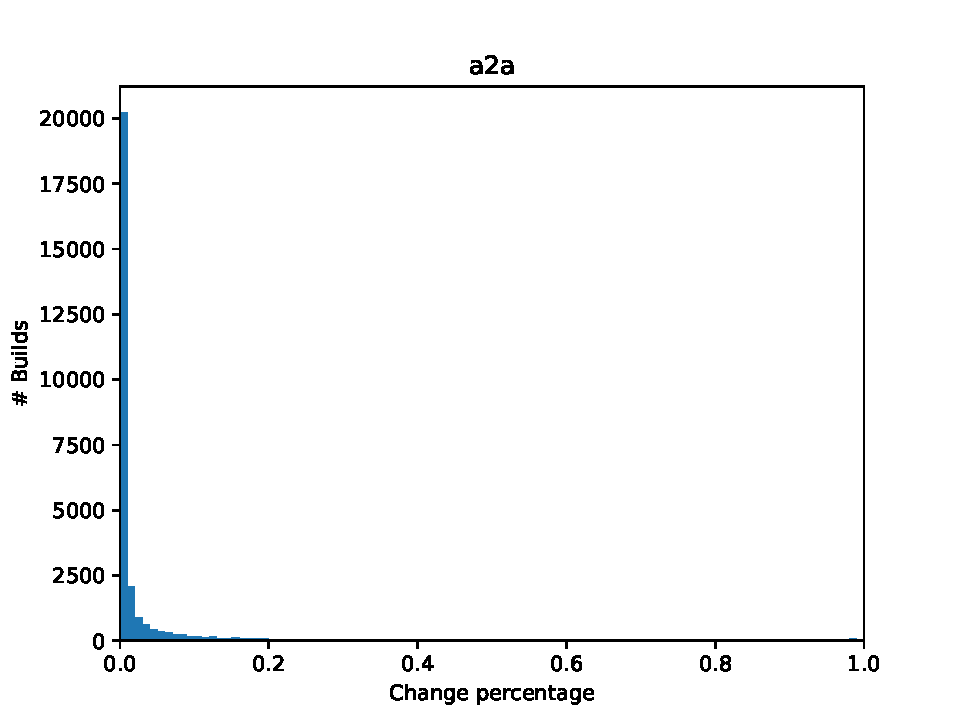
\includegraphics[width=2.3in]{assets/a2a.pdf}
		\caption{a2a}
		\label{a2aHist}
	\end{subfigure}%
	\begin{subfigure}{2.3in}
		\centering
		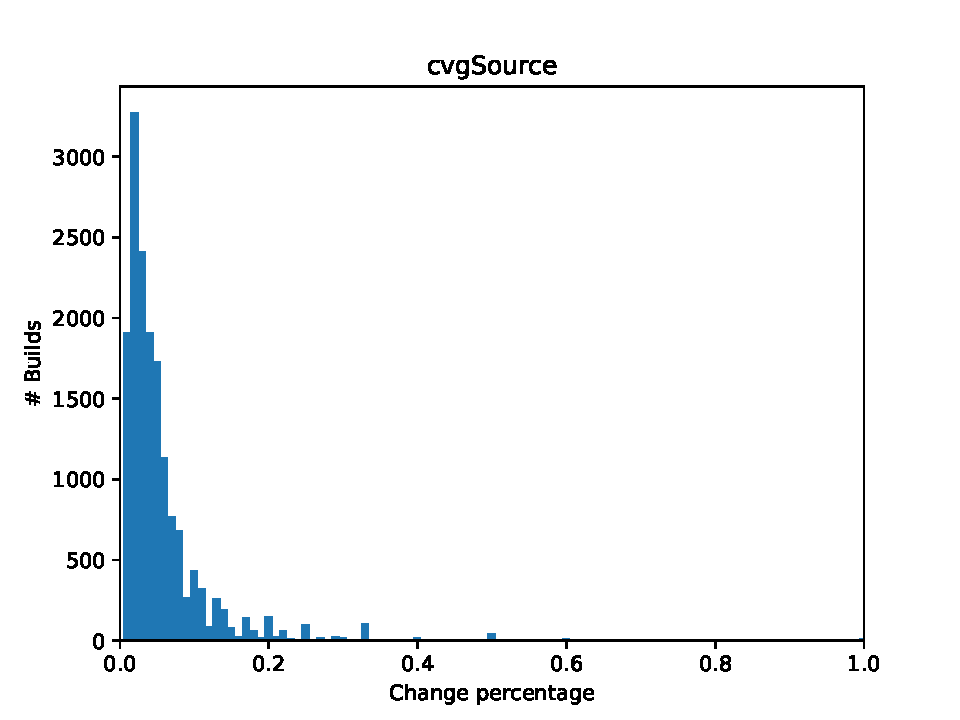
\includegraphics[width=2.3in]{assets/cvgSource.pdf}
		\caption{cvg src}
		\label{cvgHist}
	\end{subfigure}
	\caption{Histograms metric over all projects}
	\label{fig:histograms}
	
\end{figure*}

\section{Results}

This section presents the findings with the proposed methodology. First, the projects under study are introduced, then calculated metrics are evaluated and, eventually, the correlation between the metrics and the build outcomes is shown.

\subsection{Evaluation of Architecture Metrics}

p values are all 0 

\begin{table}
	\scalebox{0.85}{
	\begin{tabular}{ | c | c | c | c | c | c | c | c | c | }
		\hline
		& \#V & \#E & A. Inst & R. Inst & deg & a2a & cvg src & cvg tar \\
		\hline
		\#V & 1 & 0.93 & 0.58 & 0.59 & 0.69 & 0.23 & 0.45 & 0.49 \\
		\#E & 0.93 & 1 & 0.63 & 0.71 & 0.83 & 0.25 & 0.51 & 0.55 \\
		A. Inst & 0.58 & 0.63 & 1 & 0.81 & 0.43 & 0.2 & 0.44 & 0.46 \\
		R. Inst & 0.59 & 0.71 & 0.81 & 1 & 0.56 & 0.22 & 0.48 & 0.52 \\
		deg & 0.69 & 0.83 & 0.43 & 0.56 & 1 & 0.18 & 0.41 & 0.46 \\
		a2a & 0.23 & 0.25 & 0.2 & 0.22 & 0.18 & 1 & 0.38 & 0.37 \\
		cvg src & 0.45 & 0.51 & 0.44 & 0.48 & 0.41 & 0.38 & 1 & 0.91 \\
		cvg tar & 0.49 & 0.55 & 0.46 & 0.52 & 0.46 & 0.37 & 0.91 & 1 \\
		\hline
	\end{tabular}
	}
\end{table}


We have extracted 8 architecture change metrics. 
Table~\ref{tableMetric} shows the number of percentage of builds that show changes using the corresponding metric, i.e. the number of builds with a value greater than 0.
We can see that most builds show no change.
This is to be expected, since most changes in the system should not be architectural changes. 
Only a2a has more changing builds than non-changing builds. 
However, an investigation of these changes in Figure~\ref{a2aHist} show that most of them have a really small a2a value. 
Most other plots in Figure \ref{fig:histograms} show that for the other metrics, most changes are quite small as well, with only few big architectural changes. 
Only the number of nodes shown in Figure \ref{numNodesHist} has more widespread changes.
This could be due to the nature of the reconstruction process. ~\sn{I don't understand the next part. Please rewrite} Since we enforce a minimum number of ten nodes per architecture in the package-architecture reconstruction, we cannot have nine only nine modules. If the architecture is now changing from ten to nine, another layer of module separation is exectured. This will result in a change that is way bigger, because most packages will have more than one sub package. So the change will be most likely from ten to something above 18. The effects of this red line are not as bad as they sound, because the node degree and number of edges metrics are in the expected norm, so that it is indicated that the few outliers do not affect the results badly.

Before using the calculated metrics in further analyses, we need to ensure that our chosen metrics make sense in practice and do not all measure the exact same aspect of architectural evolution. Thus, we calculate the Pearson correlation between all the metrics we use, shown in Table \ref{tableMetricCorr}. All p values for these correlations were equal or close to 0; the highest p value we got from all the cross-metric correlations is $3.7^{-102}$. 
We consider a correlation above $60\%$ as highly correlated, and everything below $30\%$ as low correlation.
The results show that the package metrics (i.e. every metric that is calculated on the package architecture) are highly correlated, all with correlation values above $0.6$ up to $0.92$. a2a does not have any strong correlation with any of the other metrics (all values between $0.10-0.17$), while cvg shows low to medium correlation with the package metrics. 
These correlations suggest that all metrics are truly an indicator for architectural change if we assume that at least one of them is, since the p-values do not leave any doubt that the metrics are dependent.
But, as expected, the correlation is not over the roof top, because the metrics look at different angles of architectural change. But since they all look at change, they have to be correlated somehow. 
a2a and cvg highlight the change at the module level, whereas the Martin's metrics focus on the relationship between the modules. This strengthens our confidence in the chosen tool chain. ~\sn{you somehow say they are dependent but then say they look at disjunct types of changes.. can you revise the text to make the poitn clearer} \jk{better?}


\subsection{Relationship Between Architectural Changes and Build Outcome}

Around $16\%$ of all builds that had architectural changes failed ($P(f|c)$). Of course, depending on the change threshold taken, this number ranges. But all metrics showed at least at some point these $16\%$. The complete range of the values is between $8\%$ and $18\%$. 
If we check for the probability of change under the condition that the build failed ($P(c|f)$), we get a range from $0\%$ up to $60\%$, based on the metric and the change threshold. For the package metrics, the probability was almost always low, but the ARCADE metrics have more interesting results. First, the probability drastically decreases as the change threshold increases. If we look at the probability of architectural change according to the a2a metric and we consider every change (i.e. change threshold at $0.0$, then we end up with a $61\%$ probability. Of course, this is natural since we do not change the number of failing builds but the number of considered changes when we change the threshold of what we consider a change. 
Because of the constant values around $p(f|c) = 16\%$ and peak values for $p(c|f)$ with $61\%$ for a2a and $35-36\%$ for cvg, we are led to the conclusion that there is the possibility for correlation between the data.

\subsection{Correlation}

\begin{table*}
\centering
\caption{All Correlation Values}
\label{tab_corr}
\npdecimalsign{.}
\nprounddigits{2}
\scalebox{0.47}{
\begin{tabular}{l|n{5}{2}n{5}{2}|n{5}{2}n{5}{2}|n{5}{2}n{5}{2}|n{5}{2}n{5}{2}|n{5}{2}n{5}{2}|n{5}{2}n{5}{2}|n{5}{2}n{5}{2}|n{5}{2}n{5}{2}|}
Measurement & \text{\#V} && \text{\#E} && \text{Abs Inst} && \text{Rel Inst} && \text{deg} && \text{a2a} && \text{cvg}_\text{src} && \text{cvg}_\text{tar} &\\
& \text{corr} & \text{p} & \text{corr} & \text{p} & \text{corr} & \text{p} & \text{corr} & \text{p} & \text{corr} & \text{p} & \text{corr} & \text{p} & \text{corr} & \text{p} & \text{corr} & \text{p} \\
M vs Out       & -0.0000289145095637297 & 0.9948657092 & -0.0040298171 & 0.3698046118 & 0.0022653911  & 0.614146536  & -0.0057396951 & 0.2014682521 & -0.003851668  & 0.3913388604 & 0.0060641633  & 0.1771469193 & -0.0015756005 & 0.7258508615 & 0.0030200493  & 0.5015114541 \\
Ch 0 vs Out    & 0.0037602406          & 0.40267999   & 0.0032534794  & 0.4690266043 & 0.0300417962  & 2.27E-11     & 0.0030826184  & 0.4926889377 & 0.003094775   & 0.4909845061 & 0.034025072   & 3.61E-14     & 0.0189688678  & 2.42E-05     & 0.0227871875  & 3.94E-07     \\
Ch 0.01 vs Out & 0.0037602406          & 0.40267999   & 0.0012253092  & 0.7850894744 & 0.0127556787  & 0.0045270517 & 0.0019504687  & 0.6642323737 & -0.0014232955 & 0.7514298417 & 0.0102065616  & 0.0231149506 & 0.0206062693  & 4.51E-06     & 0.0236436461  & 1.42E-07     \\
Ch 0.02 vs Out & 0.0031333182         & 0.4856015219 & 0.0018544765  & 0.6798161029 & 0.0050642625  & 0.259717611  & -0.0027345375 & 0.5428078692 & 0.0002033934  & 0.9638959225 & 0.0077270799  & 0.085489307  & 0.016272552   & 0.0002926778 & 0.0213934969  & 1.92E-06     \\
Ch 0.03 vs Out                       & 0.0042190307                                & 0.3477567045                      & 0.0025605165                       & 0.5687835943                      & 0.0051882236  & 0.2482350538 & -0.0041097287 & 0.3603890768 & 0.0010919066  & 0.8080023965 & 0.0059742246  & 0.1836581701 & 0.0017611543  & 0.695098722  & 0.0087355843  & 0.0518784109 \\
Ch 0.04 vs Out                       & 0.0014490784                                & 0.7470795668                      & 0.0020395931                       & 0.6498922276                      & 0.0034026824  & 0.4488886327 & -0.0054550591 & 0.2247353518 & -0.0019714809 & 0.66084016   & 0.0069417541  & 0.1223690168 & 0.0058374296  & 0.1938989762 & 0.0125420655  & 0.0052489265 \\
Ch 0.05 vs Out                       & 0.0017918002                                & 0.6900660344                      & 0.0008905774                       & 0.8428901275                      & 0.0017189572  & 0.7020503438 & -0.0029689602 & 0.508776798  & -0.0008301001 & 0.8534339153 & 0.0091980298  & 0.0406517255 & 0.0032638886  & 0.4676056457 & 0.0105551932  & 0.0188176577 \\
Ch 0.1 vs Out                        & 0.0046535893                                & 0.3003599078                      & -0.0006015224                      & 0.8935063071                      & -0.002895869  & 0.5192661731 & -0.0043635146 & 0.3314961078 & -0.0015458722 & 0.7308206743 & 0.0085253412  & 0.0577818774 & -0.0044030985 & 0.3271284282 & -0.0029238508 & 0.5152373366 \\
Ch 0.2 vs Out                        & 0.0044235475                                & 0.3248867858                      & 0.0003357234                       & 0.9404412801                      & -0.0037729688 & 0.4010894098 & -0.0037729688 & 0.4010894098 & -0.0081461641 & 0.0698381676 & 0.0035337901  & 0.431605414  & -0.0037605771 & 0.4026378941 & -0.0044506456 & 0.3219317189 \\
Ch 0.5 vs Out                        & -0.0051725129                               & 0.2496703567                      & -0.0073164419                      & 0.1034621595                      & -0.0009041882 & 0.8405241716 & -0.0076433044 & 0.0889415141 & -0.002667838  & 0.5526937937 & 0.0075762872  & 0.0917713638 & -0.0007291211 & 0.8710964557 & 0.00187497    & 0.6764773189 \\
M vs Bef 2                           & -0.0034760989                               & 0.4391717986                      & -0.004882384                       & 0.2772317221                      & 0.0004389442  & 0.9221823715 & -0.0070264809 & 0.1178807512 & -0.0026812148 & 0.5507121276 & 0.0105902894  & 0.0184288366 & 0.0022399117  & 0.6181437206 & 0.006027498   & 0.1797890805 \\
M vs Nxt 2                           & -0.0029263758                               & 0.5148830728                      & -0.0053631581                      & 0.2326519731                      & 0.017532964   & 9.53E-05     & -0.0043752283 & 0.3302094794 & -0.0041943905 & 0.3505893069 & 0.0064904345  & 0.1486174381 & -0.0069571586 & 0.1215493441 & -0.0039611395 & 0.3780271137 \\
Ch 0 vs Bef 2                        & 0.001165378                                 & 0.7953654283                      & -0.004353406                       & 0.3326272637                      & 0.0312507388  & 3.49E-12     & 0.0033189796  & 0.4601341245 & -0.003444723  & 0.4433135019 & 0.0347050873  & 1.11E-14     & 0.0197292579  & 1.13E-05     & 0.0240889517  & 8.25E-08     \\
Ch 0 vs Nxt 2                        & 0.0033557122                                & 0.455183844                       & 0.0038970759                       & 0.3857886057                      & 0.0096731539  & 0.0313369758 & 0.0019631654  & 0.6621881811 & 0.0032817437  & 0.465182831  & 0.0362237394  & 7.38E-16     & 0.017557845   & 9.32E-05     & 0.0189810208  & 2.39E-05     \\
Ch 0.01 vs Bef 2                     & 0.001165378                                 & 0.7953654283                      & -0.0035324246                      & 0.4317927043                      & 0.0110692852  & 0.0137589785 & 0.0018675562  & 0.6776905762 & -0.0044354506 & 0.3235963447 & 0.0094729988  & 0.0350119146 & 0.0217337849  & 1.32E-06     & 0.0255680171  & 1.26E-08     \\
Ch 0.01 vs Nxt 2                     & 0.0033557122                                & 0.455183844                       & 0.0023093549                       & 0.6072958841                      & 0.0020778021  & 0.6437901966 & -0.0028227793 & 0.5298741775 & 0.0013881961  & 0.757369493  & 0.0093437666  & 0.0375752191 & 0.0194328359  & 1.52E-05     & 0.0197393939  & 1.12E-05     \\
Ch 0.02 vs Bef 2                     & 0.000478508                                 & 0.9151937368                      & -0.0021968871                      & 0.6249068865                      & 0.0040788768  & 0.3640158922 & -0.00301242   & 0.5026015369 & 0.0009856013  & 0.8263842814 & 0.0087026519  & 0.0527731347 & 0.0149773701  & 0.0008581208 & 0.0222803785  & 7.09E-07     \\
Ch 0.02 vs Nxt 2                     & 0.0031108808                                & 0.4887400356                      & 0.0003070356                       & 0.9455234254                      & 0.005277331   & 0.240213048  & -0.0031569907 & 0.4823201246 & 0.0038406674  & 0.3927026363 & 0.0075551222  & 0.0926886504 & 0.0147164807  & 0.001055633  & 0.0160521678  & 0.0003534978 \\
Ch 0.03 vs Bef 2                     & 0.0021719985                                & 0.628833709                       & -0.0001993733                      & 0.9646097702                      & 0.0038629726  & 0.3899597429 & -0.0025385764 & 0.5721080047 & 0.0004752246  & 0.9157734927 & 0.0078410066  & 0.0809835519 & -0.0003458187 & 0.9386550467 & 0.0074017768  & 0.0995057061 \\
Ch 0.03 vs Nxt 2                     & 0.0031793912                                & 0.4792179223                      & 0.0019668539                       & 0.6615929565                      & 0.0030620172  & 0.4955932808 & -0.007704632  & 0.0864081992 & 0.0023433115  & 0.6020225876 & 0.0065880516  & 0.142605481  & -0.0023767613 & 0.5968482675 & 0.0010057284  & 0.822897061  \\
Ch 0.04 vs Bef 2                     & -0.0008678892                               & 0.8468455138                      & 0.0005805042                       & 0.8972084151                      & 0.0017770198  & 0.692497485  & -0.005794707  & 0.1971906917 & -0.0006214115 & 0.8900093808 & 0.0094241788  & 0.0359621478 & 0.0052896641  & 0.2391160179 & 0.0123774698  & 0.0058753923 \\
Ch 0.04 vs Nxt 2                     & -0.0012379213                               & 0.7829367958                      & 0.0015612085                       & 0.7282606808                      & 0.0012004491  & 0.7893501053 & -0.0057481551 & 0.200813746  & -0.0002023296 & 0.9640853632 & 0.0079239505  & 0.0778217224 & 0.0046325317  & 0.3025621055 & 0.0053880351  & 0.2304923016 \\
Ch 0.05 vs Bef 2                     & -0.0001461219                               & 0.9740583506                      & 0.0002807733                       & 0.9501767347                      & 0.0016101182  & 0.7201002685 & -0.0050981608 & 0.2565512821 & 0.0026036428  & 0.5622990811 & 0.0132042547  & 0.0032961791 & 0.0035505918  & 0.4294280661 & 0.0104544833  & 0.0199832722 \\
Ch 0.05 vs Nxt 2                     & -0.0005283513                               & 0.9063986999                      & 0.0007504366                       & 0.8673650786                      & -0.0019034063 & 0.6718612828 & -0.0026308406 & 0.5582231663 & 0.0011851238  & 0.7919771363 & 0.0100481448  & 0.0253369795 & 0.0001808438  & 0.967897029  & 0.0034858778  & 0.4378855237 \\
Ch 0.1 vs Bef 2                      & 0.0048938053                                & 0.2761094051                      & 0.0033529173                       & 0.4555594338                      & -0.0039019582 & 0.3851937011 & -0.0043227285 & 0.3360454529 & 0.0047147992  & 0.2940570051 & 0.0114052567  & 0.0111401644 & -0.0055313296 & 0.2183296249 & -0.0010734342 & 0.8111924177 \\
Ch 0.1 vs Nxt 2                      & 0.004296711                                 & 0.3389620551                      & 0.000394848                        & 0.9299786843                      & -0.0045662495 & 0.3095324545 & -0.0045662495 & 0.3095324545 & 0.0006033523  & 0.8931864217 & 0.0082733668  & 0.0655875595 & -0.0124771068 & 0.0054891531 & -0.0094601529 & 0.0352598464 \\
Ch 0.2 vs Bef 2                      & 0.0011970423                                & 0.7899338812                      & 0.0027825075                       & 0.5357610771                      & 0.0001366939  & 0.9757316058 & 0.0001366939  & 0.9757316058 & -0.0021270067 & 0.635959004  & 0.0049562128  & 0.2700316625 & -0.0027872945 & 0.5350595936 & -0.0035918123 & 0.4240908327 \\
Ch 0.2 vs Nxt 2                      & 0.0014224411                                & 0.7515789926                      & 4.82E-06                           & 0.9991437275                      & 0.0004770793  & 0.9154468554 & -0.0075091802 & 0.0946938395 & -0.005751846  & 0.2005247268 & 0.0020158749  & 0.6537026647 & -0.0105468995 & 0.0189135597 & -0.0100243402 & 0.0256859088 \\
Ch 0.5 vs Bef 2                      & -0.0076648083                               & 0.0880465058                      & -0.0059859513                      & 0.1828081242                      & 0.0002509771  & 0.95545871   & -0.0067940629 & 0.1305363277 & -0.0032287608 & 0.4724194275 & 0.0085513929  & 0.0570263481 & 0.0023095162  & 0.6072707773 & 0.0062150047  & 0.1666235675 \\
Ch 0.5 vs Nxt 2                      & -0.0048590507                               & 0.2795342279                      & -0.0070288705                      & 0.117755857                       & 0.0219650316  & 1.01E-06     & -0.0033190938 & 0.460123213  & -0.003223201  & 0.4731823855 & 0.0073888289  & 0.100099165  & -0.0039457553 & 0.3798821235 & -0.0025280664 & 0.5737000067 \\
M vs Bef 3                           & -0.003517936                                & 0.4336885643                      & -0.0044699912                      & 0.3198474835                      & 0.0332526133  & 1.34E-13     & 0.0024064705  & 0.5922733568 & -0.0015390242 & 0.731974903  & 0.0110820364  & 0.0136513825 & 5.85E-05      & 0.9896127406 & 0.0034864055  & 0.437820795  \\
M vs Nxt 3                           & -0.0041109137                               & 0.3602651456                      & -0.0066925109                      & 0.1363847418                      & 0.0114068102  & 0.0111299775 & 0.0024555595  & 0.5847435775 & -0.0044763988 & 0.3191542641 & 0.0056755608  & 0.2065647671 & -0.008103318  & 0.0713303815 & -0.006387091  & 0.1551951279 \\
Ch 0 vs Bef 3                        & 0.0005437047                                & 0.9036927602                      & -0.0030780689                      & 0.4933407032                      & 0.0117963587  & 0.0086574842 & 0.0031483022  & 0.4835307305 & -0.0020163295 & 0.6536329509 & 0.037333146   & 9.48E-17     & 0.0215866735  & 1.55E-06     & 0.0258345466  & 8.91E-09     \\
Ch 0 vs Nxt 3                        & 0.0045061195                                & 0.3159517814                      & 0.0024371305                       & 0.5875651929                      & 0.0039423029  & 0.3803039911 & 0.0001898845  & 0.9662934203 & 0.0026020878  & 0.5625365044 & 0.0373825134  & 8.64E-17     & 0.0176271406  & 8.74E-05     & 0.0190448505  & 2.25E-05     \\
Ch 0.01 vs Bef 3                     & 0.0005437047                                & 0.9036927602                      & -0.0033536942                      & 0.4554595622                      & 0.0045129093  & 0.3152231254 & -0.0014440027 & 0.7479427304 & -0.0025102642 & 0.5764052162 & 0.0077564779  & 0.0843154305 & 0.0236907783  & 1.34E-07     & 0.027530333   & 8.91E-10     \\
Ch 0.01 vs Nxt 3                     & 0.0045061195                                & 0.3159517814                      & 0.0019178549                       & 0.6695205953                      & 0.0072720134  & 0.1055852699 & 0.0004731327  & 0.9161437144 & 0.0019882759  & 0.6581434739 & 0.0069440978  & 0.122254193  & 0.0193568744  & 1.65E-05     & 0.020296901   & 6.26E-06     \\
Ch 0.02 vs Bef 3                     & -0.0001988864                               & 0.9646964883                      & -0.001432939                       & 0.7498091226                      & 0.0024452614  & 0.5863195102 & -0.0026741727 & 0.5517631564 & 0.0033711251  & 0.4531202389 & 0.0060219564  & 0.1801940068 & 0.0155710232  & 0.000529372  & 0.0222492334  & 7.34E-07     \\
Ch 0.02 vs Nxt 3                     & 0.003247171                                 & 0.4699023761                      & 0.0003693122                       & 0.9344972597                      & 0.0070258793  & 0.1179159209 & -0.0038469223 & 0.391937058  & 0.0047769424  & 0.2877445961 & 0.0050829306  & 0.2579796614 & 0.0144595654  & 0.0012906669 & 0.0141969563  & 0.00157988   \\
Ch 0.03 vs Bef 3                     & 0.0019723964                                & 0.6607021503                      & -0.000248138                       & 0.9559620438                      & -8.01E-06     & 0.9985768541 & -0.0064552937 & 0.1508325282 & 0.001228987   & 0.7844666858 & 0.0063253446  & 0.1592267815 & -0.0012485352 & 0.7811250497 & 0.0057711928  & 0.1990192699 \\
Ch 0.03 vs Nxt 3                     & 0.0036376568                                & 0.4182053797                      & 0.0013400421                       & 0.7655371961                      & 0.0049474335  & 0.2708859133 & -0.0040868878 & 0.3630793473 & 0.0020571829  & 0.6470870405 & 0.0045903482  & 0.3069909017 & -0.0027764329 & 0.536656029  & -0.0013172051 & 0.7694187913 \\
Ch 0.04 vs Bef 3                     & -0.0002960432                               & 0.9474714413                      & 0.0015435118                       & 0.7312235847                      & 0.0003652207  & 0.9352213384 & -0.0050277354 & 0.263184651  & 0.0016658929  & 0.710836048  & 0.0077238119  & 0.0856311473 & 0.0048131578  & 0.2841055886 & 0.0103222044  & 0.0216074688 \\
Ch 0.04 vs Nxt 3                     & -0.0008673309                               & 0.8469443334                      & 0.001535677                        & 0.7325354588                      & -0.000642259  & 0.8863451379 & -0.0041479453 & 0.3559544645 & -0.0006475684 & 0.8854120288 & 0.0047525612  & 0.2902121121 & 0.0022721955  & 0.6130936426 & 0.0025950346  & 0.5635960614 \\
Ch 0.05 vs Bef 3                     & 0.0003729448                                & 0.9338544484                      & 0.0018784127                       & 0.6759263248                      & -0.0014642322 & 0.7445339284 & -0.0022771254 & 0.612323539  & 0.0048566297  & 0.2797787236 & 0.0104413411  & 0.020140862  & 0.0031134104  & 0.4883910415 & 0.0080568873  & 0.0729673265 \\
Ch 0.05 vs Nxt 3                     & 0.0001200364                                & 0.9786884168                      & 0.0008094228                       & 0.8570492397                      & -0.0051553979 & 0.2512549048 & -0.0051553979 & 0.2512549048 & 0.0017935638  & 0.6897857358 & 0.0070949015  & 0.1143492825 & -0.001807732  & 0.6874640649 & -0.0011635134 & 0.7956875992 \\
Ch 0.1 vs Bef 3                      & 0.0074831368                                & 0.0958439582                      & 0.0047333069                       & 0.2921707937                      & 0.000131444   & 0.9766636289 & 0.000131444   & 0.9766636289 & 0.0065627255  & 0.1441510532 & 0.0096250188  & 0.0321908576 & -0.0093630756 & 0.0371842807 & -0.0038709773 & 0.388983026  \\
Ch 0.1 vs Nxt 3                      & 0.0033709595                                & 0.4531424335                      & 0.0007256233                       & 0.8717133127                      & 0.0002767976  & 0.9508828172 & -0.0065186902 & 0.1468699203 & 0.0022068241  & 0.6233455223 & 0.0057521268  & 0.2005072907 & -0.0171748995 & 0.0001321377 & -0.0149473263 & 0.0008790854 \\
Ch 0.2 vs Bef 3                      & 0.0021440946                                & 0.6332522262                      & 0.0023220306                       & 0.6053286401                      & -0.000408095  & 0.9276380275 & -0.0079341882 & 0.0774475028 & 0.0006156758  & 0.8910193352 & 0.0032429116  & 0.4704850868 & -0.0078323861 & 0.0813211377 & -0.0069336961 & 0.1228148015 \\
Ch 0.2 vs Nxt 3                      & -0.0007668796                               & 0.8644880452                      & -0.0001345658                      & 0.9761095448                      & 0.0252179146  & 1.99E-08     & -0.0013828894 & 0.7582751241 & -0.0033766412 & 0.4523813562 & -0.0009716445 & 0.8288061401 & -0.0125979308 & 0.0050520553 & -0.0130466157 & 0.0036894642 \\
Ch 0.5 vs Bef 3                      & -0.0091865203                               & 0.0409099743                      & -0.0054455958                      & 0.2255546464                      & 0.031939644   & 1.16E-12     & -0.0024373226 & 0.5875432857 & -0.0036453432 & 0.4172225541 & 0.0076142925  & 0.0901638591 & 0.0004820211  & 0.9145743453 & 0.0040878575  & 0.3629654909 \\
Ch 0.5 vs Nxt 3                      & -0.0043701324                               & 0.3307779319                      & -0.0079289029                      & 0.0776391566                      & 0.010906251   & 0.0152185598 & 0.004124061   & 0.3587406864 & -0.0036395775 & 0.4179596543 & 0.0061544517  & 0.1707978425 & -0.0052853318 & 0.2395057155 & -0.004293121  & 0.3393706406 \\
M vs Bef 5                           & -0.0027555055                               & 0.5397388461                      & -0.0040964417                      & 0.3619683272                      & 0.0136048837  & 0.002463785  & 0.0048392152  & 0.2815163371 & -0.0008003543 & 0.8586366853 & 0.0111043773  & 0.013464898  & -0.0035597591 & 0.4282517152 & -0.0013129704 & 0.7701437114 \\
M vs Nxt 5                           & -0.005867585                                & 0.1916286281                      & -0.0074572696                      & 0.0970040866                      & 0.0020852247  & 0.6426163451 & 0.0020952838  & 0.6410133911 & -0.0054978784 & 0.2211407951 & 0.0051712143  & 0.2498131613 & -0.0111953667 & 0.0127211737 & -0.0100928785 & 0.0246967142 \\
Ch 0 vs Bef 5                        & 0.0034436553                                & 0.4434686313                      & -0.0008779481                      & 0.8450974188                      & 0.0067188382  & 0.1348573461 & 0.0004816262  & 0.9146457832 & 0.0007633471  & 0.8651089679 & 0.0402428094  & 3.27E-19     & 0.0221323544  & 8.40E-07     & 0.0259472885  & 7.68E-09     \\
Ch 0 vs Nxt 5                        & 0.0028152485                                & 0.5309849747                      & -0.0029718605                      & 0.5083842891                      & 0.0052696865  & 0.240909053  & 0.0013906975  & 0.7569532011 & -0.0020311449 & 0.6512625379 & 0.0378653698  & 3.47E-17     & 0.0200293903  & 8.28E-06     & 0.0212200445  & 2.33E-06     \\
Ch 0.01 vs Bef 5                     & 0.0034436553                                & 0.4434686313                      & -0.0015990582                      & 0.7219509113                      & 0.0047523946  & 0.2902387678 & -0.0011924914 & 0.7907200948 & 0.0003504264  & 0.9378412146 & 0.0096538011  & 0.0316823913 & 0.0251871546  & 2.07E-08     & 0.02743769    & 1.01E-09     \\
Ch 0.01 vs Nxt 5                     & 0.0028152485                                & 0.5309849747                      & -0.0020307472                      & 0.6513262982                      & 0.0055120757  & 0.2199504754 & -0.0035901561 & 0.4243185606 & 0.0001033027  & 0.9816591699 & 0.003254501   & 0.4689094828 & 0.0214980962  & 1.71E-06     & 0.023601115   & 1.50E-07     \\
Ch 0.02 vs Bef 5                     & 0.0030962696                                & 0.4907970541                      & -0.0003420562                      & 0.9393230177                      & 0.0013149294  & 0.7698104192 & -0.0076976719 & 0.0867022837 & 0.0058837722  & 0.1904061014 & 0.0082483133  & 0.0664167438 & 0.0132862476  & 0.0031081381 & 0.0195307815  & 1.38E-05     \\
Ch 0.02 vs Nxt 5                     & 0.0020665171                                & 0.6456018867                      & -0.0018516679                      & 0.6802894196                      & 0.0054868539  & 0.2220682782 & -0.0044472847 & 0.3223216924 & 0.0034622154  & 0.4410155558 & 0.0011378153  & 0.8001074163 & 0.0128425067  & 0.0042622181 & 0.0152126232  & 0.0007102433 \\
Ch 0.03 vs Bef 5                     & 0.0053832312                                & 0.2309223552                      & 7.76E-05                           & 0.9862244325                      & 7.25E-05      & 0.9871328098 & -0.0059279991 & 0.1870951879 & 0.0031815222  & 0.4789366864 & 0.0080444143  & 0.0734180777 & -0.0064595985 & 0.1505685763 & 0.0012069715  & 0.7882390231 \\
Ch 0.03 vs Nxt 5                     & 0.003525034                                 & 0.4327707462                      & -0.0002527792                      & 0.9551401191                      & 0.00025841    & 0.9541419334 & -0.001554458  & 0.729397297  & 0.0014088787  & 0.7538778277 & 0.0014814936  & 0.7416342643 & -0.0070018543 & 0.1191851132 & -0.0035500871 & 0.4295076331 \\
Ch 0.04 vs Bef 5                     & 0.0030461223                                & 0.4978466127                      & 0.0030845121                       & 0.4924450599                      & -0.0011140941 & 0.8041891964 & -0.004852232  & 0.2802240993 & 0.0038256064  & 0.3945756121 & 0.0098867261  & 0.02779033   & 0.0014822367  & 0.7415093008 & 0.0066021583  & 0.1417644137 \\
Ch 0.04 vs Nxt 5                     & -0.0003077347                               & 0.9454012279                      & 0.0003923335                       & 0.9304255645                      & -0.0022022102 & 0.6240788999 & -0.0022022102 & 0.6240788999 & -0.0002672632 & 0.9525726478 & 0.0026312923  & 0.5581675144 & -0.0017030989 & 0.7046835668 & 0.000293311   & 0.9479565869 \\
Ch 0.05 vs Bef 5                     & 0.0029871362                                & 0.5062071633                      & 0.0037760976                       & 0.4007227838                      & -0.0013478875 & 0.7642096928 & -0.0013478875 & 0.7642096928 & 0.0063354452  & 0.1585703117 & 0.0117651175  & 0.0088372888 & -0.0002876103 & 0.9489666924 & 0.0043942925  & 0.328121244  \\
Ch 0.05 vs Nxt 5                     & -0.0004665302                               & 0.917311349                       & 0.0008750031                       & 0.8456104799                      & 0.0035819632  & 0.4253999448 & -0.0036495321 & 0.4167204508 & 0.0031348141  & 0.485415272  & 0.0048910451  & 0.2763948975 & -0.0065106169 & 0.1473711081 & -0.0029437992 & 0.5123963889 \\
Ch 0.1 vs Bef 5                      & 0.0074446193                                & 0.097572193                       & 0.0033256447                       & 0.4592472634                      & -0.0061703924 & 0.1697227447 & -0.0130865553 & 0.003588428  & 0.0083221279  & 0.0640217884 & 0.0084411933  & 0.0603092207 & -0.0139428778 & 0.0019158157 & -0.0084018178 & 0.0615167216 \\
Ch 0.1 vs Nxt 5                      & 0.0035296457                                & 0.4321690096                      & 0.001740044                        & 0.6985877723                      & 0.0291919145  & 8.17E-11     & -0.0002527556 & 0.9551465613 & 0.0029362369  & 0.5134804378 & 0.0030403343  & 0.4986637256 & -0.0204995335 & 5.06E-06     & -0.0199937376 & 8.59E-06     \\
Ch 0.2 vs Bef 5                      & 0.0019549066                                & 0.6635312802                      & 0.0035147569                       & 0.434113468                       & 0.0288972807  & 1.26E-10     & -0.0070186425 & 0.1183208839 & 0.0037945622  & 0.3984234638 & 0.0022558889  & 0.6156510948 & -0.0126139471 & 0.0049973609 & -0.0126233555 & 0.0049649697 \\
Ch 0.2 vs Nxt 5                      & -0.0044422443                               & 0.3228704254                      & -0.0007833943                      & 0.8616016959                      & 0.0144248958  & 0.0013268724 & 0.0065922814  & 0.142381491  & -0.0021012721 & 0.640059939  & -0.0013615261 & 0.7618956013 & -0.0182166033 & 5.03E-05     & -0.0176203425 & 8.80E-05     \\
Ch 0.5 vs Bef 5                      & -0.0074590105                               & 0.0969261121                      & -0.0032621855                      & 0.4678604457                      & 0.0067650305  & 0.1322154306 & -0.0010265919 & 0.8193002954 & -0.0042891348 & 0.3398290268 & 0.0080514087  & 0.0731682864 & -0.0013627815 & 0.7616826929 & -0.0004624758 & 0.918027418  \\
Ch 0.5 vs Nxt 5                      & -0.0061576967                               & 0.1705810475                      & -0.0109890972                      & 0.0144621803                      & 0.0098134746  & 0.0289754172 & 0.0068504814  & 0.1273991896 & -0.0042810968 & 0.34073482   & 0.0028068502  & 0.5322111757 & -0.0087025241 & 0.0527837863 & -0.006847911  & 0.1275228272 \\
M vs Bef 10                          & 0.0011720458                                & 0.7942370749                      & -0.0005514585                      & 0.9023330115                      & 0.0016584195  & 0.7120947426 & -0.0044648155 & 0.3204423408 & 0.0034506751  & 0.4425629424 & 0.0099889674  & 0.0262241852 & -0.0058482461 & 0.1931192221 & -0.004943465  & 0.2713043474 \\
M vs Nxt 10                          & -0.0096331076                               & 0.0320584291                      & -0.0106183997                      & 0.0181299767                      & 0.0104617052  & 0.0199077984 & 0.0039675544  & 0.3772937938 & -0.0074272707 & 0.0983725989 & 0.0085823729  & 0.0561526095 & -0.0139378666 & 0.0019240659 & -0.0129361808 & 0.0039922083 \\
Ch 0 vs Bef 10                       & 0.0050383583                                & 0.2622110283                      & 0.0007659342                       & 0.8646629547                      & -1.94E-05     & 0.9965476573 & -0.0078769837 & 0.0796238279 & 0.0027074069  & 0.5468588944 & 0.0431944812  & 6.81E-22     & 0.024938014   & 2.85E-08     & 0.0286299287  & 1.86E-10     \\
Ch 0 vs Nxt 10                       & -0.0021970818                               & 0.6249041567                      & -0.0076452634                      & 0.0888854649                      & 0.0097896461  & 0.0293674997 & -0.002600462  & 0.5628082486 & -0.0073506179 & 0.1018946611 & 0.0424074421  & 3.69E-21     & 0.0239783474  & 9.47E-08     & 0.025128717   & 2.24E-08     \\
Ch 0.01 vs Bef 10                    & 0.0050383583                                & 0.2622110283                      & 0.002696567                        & 0.5484652602                      & -0.0044027382 & 0.327216849  & -0.0135900717 & 0.0024920533 & 0.0057830419  & 0.1981302721 & 0.0050724497  & 0.2589961567 & 0.0267627723  & 2.58E-09     & 0.030467205   & 1.19E-11     \\
Ch 0.01 vs Nxt 10                    & -0.0021970818                               & 0.6249041567                      & -0.0064098407                      & 0.1537584993                      & 0.0098977229  & 0.0276250883 & -0.0022570056 & 0.6154941295 & -0.0040952391 & 0.3621335076 & -0.0006313665 & 0.8882677575 & 0.0254136512  & 1.55E-08     & 0.0274915181  & 9.43E-10     \\
Ch 0.02 vs Bef 10                    & 0.0051257515                                & 0.2540246414                      & 0.001437402                        & 0.7490731917                      & -0.0039088059 & 0.3843986507 & -0.0107467685 & 0.0167787299 & 0.0121026444  & 0.0070754914 & 0.0053670373  & 0.2323519841 & 0.0148302745  & 0.0009657266 & 0.0181092463  & 5.57E-05     \\
Ch 0.02 vs Nxt 10                    & -0.0029489859                               & 0.5116748838                      & -0.007699133                       & 0.0866583893                      & -0.0016777205 & 0.7088959575 & -0.0027662304 & 0.5381825856 & -0.0002850064 & 0.9494306519 & -0.0001543039 & 0.9726085275 & 0.0135126532  & 0.0026377505 & 0.017155134   & 0.0001346631 \\
Ch 0.03 vs Bef 10                    & 0.007294714                                 & 0.1045260878                      & 0.0026979513                       & 0.5482599948                      & -0.0058337456 & 0.1942254811 & -0.009129999  & 0.042182169  & 0.0079609167  & 0.0764690929 & 0.0065484875  & 0.1450516998 & -0.0071302816 & 0.1125796764 & -0.0022390571 & 0.6183061165 \\
Ch 0.03 vs Nxt 10                    & -0.0010611337                               & 0.8133306083                      & -0.0048699387                      & 0.2784970184                      & 0.0001566785  & 0.9721871686 & 0.0001566785  & 0.9721871686 & -0.0016550054 & 0.7126611064 & 0.0013810687  & 0.7585952826 & -0.010409713  & 0.0205304148 & -0.0063944853 & 0.1547467259 \\
Ch 0.04 vs Bef 10                    & 0.0060900732                                & 0.1753469967                      & 0.0047094027                       & 0.2946489541                      & -0.0036378365 & 0.4182152815 & -0.0036378365 & 0.4182152815 & 0.0081163504  & 0.0708962991 & 0.008721617   & 0.0522780795 & 0.0012946299  & 0.7732771537 & 0.0028700622  & 0.5230381786 \\
Ch 0.04 vs Nxt 10                    & -0.0040075944                               & 0.3724981895                      & -0.0037546061                      & 0.4034327848 &&&&                     & -0.0027762308 & 0.5367144601 & 0.0036877027  & 0.4118638109 & -0.0015544956 & 0.7294041454 & -0.0007247246 & 0.8718798064          \\
Ch 0.05 vs Bef 10                    & 0.0062088999                                & 0.1670747542                      & 0.0071925289                       & 0.1094752139 &&&&                     & 0.0115833235  & 0.0099461801 & 0.0098639774  & 0.0281593014 & -0.0001285653 & 0.9771761864 & 0.0023635261  & 0.5989226982            \\
Ch 0.05 vs Nxt 10                    & -0.005254351                                & 0.2423046136                      & -0.0026981166                      & 0.5482354924  &&&&                    & -0.0006590566 & 0.8834017793 & 0.00671966    & 0.1348293331 & -0.0068530513 & 0.1272564867 & -0.0039097566 & 0.3842830301              \\
Ch 0.1 vs Bef 10                     & 0.0088107373                                & 0.0499175753                      & 0.0075833946                       & 0.0914998925 &&&&                     & 0.010165014   & 0.0236940764 & 0.005990776   & 0.1824909447 & -0.0165783367 & 0.0002247926 & -0.0139918132 & 0.0018474723         \\
Ch 0.1 vs Nxt 10                     & -0.0017994744                               & 0.6888376891                      & -0.0020582368                      & 0.6469417946 &&&&                     & -0.0001772688 & 0.9685338614 & 0.0036154395  & 0.421086658  & -0.0265166712 & 3.60E-09     & -0.0268532865 & 2.28E-09              \\
Ch 0.2 vs Bef 10                     & 0.0036575086                                & 0.4157027711                      & 0.0053241685                       & 0.236103473 &&&&                      & 0.0082184069  & 0.0674216866 & -0.0018216816 & 0.6852021501 & -0.0145653298 & 0.0011896138 & -0.0167537433 & 0.0001926759             \\
Ch 0.2 vs Nxt 10                     & -0.0088216595                               & 0.0496345242                      & -0.0041836567                      & 0.3518624329 &&&&                     & -0.0034601574 & 0.4413102274 & -0.0014584411 & 0.7455266289 & -0.0213793641 & 1.95E-06     & -0.0204603407 & 5.28E-06         \\
Ch 0.5 vs Bef 10                     & 0.0015613404                                & 0.728259719                       & 0.0016743638                       & 0.7094518998 &&&&                     & 0.0056245106  & 0.2107089728 & 0.0067594862  & 0.1325327286 & -0.0017773336 & 0.6924695227 & 0.0001965733  & 0.9651092889      \\
Ch 0.5 vs Nxt 10                     & -0.0042750334                               & 0.3414434986                      & -0.0115946009                      & 0.0098741799 &&&&                     & -0.0053901816 & 0.2303442757 & 0.0049663502  & 0.269091806  & -0.0095338792 & 0.0338714466 & -0.0081959138 & 0.0681751972         
\end{tabular}
}
\end{table*}

When calculating the correlation between architectural change and build outcome, we got the values as mentioned in table \ref{tab_corr}. As you can see some of the metrics show no correlation at all ($c < 0.4\%$ and $p > 0.25$), while the top metrics, a2a and cvg, peak at $4.3\%$ ($p = 6.8 \cdot 10^{-22}$) and $3.0\%$ ($p=1.2 \cdot 10^{-11}$). 
The threshold that controls how many previous or following builds are considered had no large impact. Only when going using a very large window, with the previous $40$ builds, do we start to see a significant rise in the correlation, as shown in Figure \ref{a2aPrevN}). However, a rise from $3\%$ to $6\%$, although it has doubled, is not that interesting. Furthermore, to consider the previous $80$ builds, where the peak occurred, is likely due to chance than to actual correlation~\sn{wouldn't the p-value have told you this?} \jk{why would it? The p-value doesnt know anything about the structure of the data}. In other words, it is improbable that code that was committed up to $80$ builds before the current one, influences the architecture. ~\sn{do you consider each of the 80 builds or literally the build 80 commits before?} \jk{each of the builds, I added "up to" to clarify}
Nevertheless, in Figure \ref{a2aPlot}, we computed the correlation values over the next $80$ builds for different change thresholds, and confirmed our intuition that the correlation is even lower than the one for the next $10$ builds after the initial peak.
The highest correlation found for a2a was the one with a change threshold of $0.0$, i.e. every little change was considered as an architectural change. However, even the strongest correlation we found, in a realistic scenario, was only $4\%$ over the next ten builds~\sn{I don't see the blue line at 4 percent or is it just hidden by the red?} \jk{just hidden, confirm the new table to check}. 

Some of the metrics have low p-values, which indicates that there is a statistically significant relationship between build outcome and those metrics. However, the detected correlation is so small that we cannot conclude this as a meaningful impact. Because taking the smallest changes into consideration increases the correlation coefficient, and the threshold for previous and following builds had no significant change on the correlation coefficient, we conclude that the stronger correlations could be noise. 
The strongest correlation was found with the a2a metric, which works on the modules and does not consider the relationship between them. Therefore, the possible correlation happens not in the interaction between the modules, but the modules themselves. Furthermore, over all correlations, the tendency was towards a positive value, with only $38\%$ negative correlation values. Because we marked no build error with a zero, this shows that change is occurring more often around failing builds, whereas a static architecture shows in the near of non-failing builds. That is, if there truly is a correlation.
~\sn{how did you conclude that?} \jk{oh youre right, thats the other way around .. my mistake. Correlation ranges from -1 to 1 and -1 is a perfect negative correlation, we have a positive one, which says if change is rising, then the build outcome is rising. And a "low build outcome" is 0 which is no error}

\begin{figure}[!t]
	\centering
	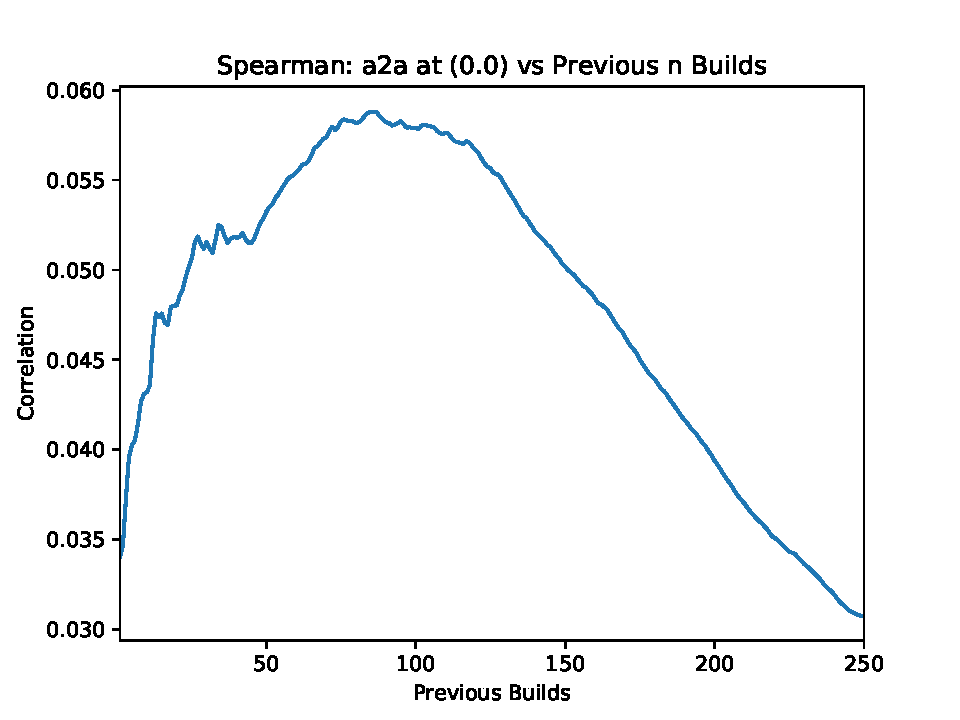
\includegraphics[width=3in]{assets/PrevN}
	\caption{a2a vs previous n builds over 0.0 threshold }
	\label{a2aPrevN}
\end{figure}

\begin{figure}[!t]
	\centering
	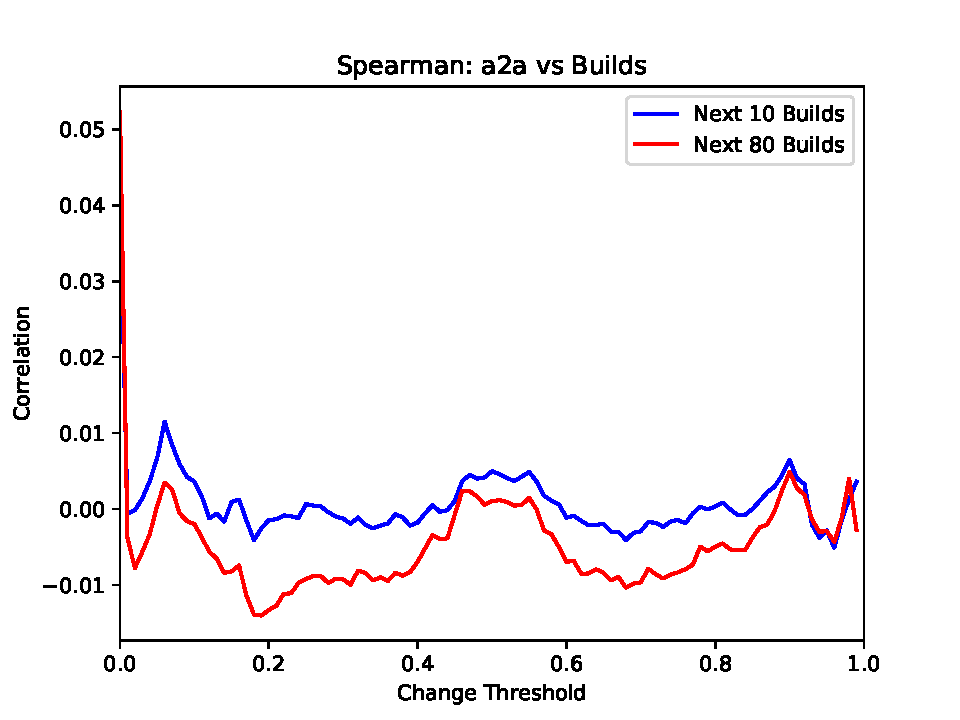
\includegraphics[width=3in]{assets/a2aCorr}
	\caption{a2a vs next ten and eighty builds over different change thresholds }
	\label{a2aPlot}
\end{figure}


\section{Discussion and Threats to Validity}

After analyzing $159$ Java projects, we found no significant correlation between architectural change and CI build outcome. Apart from there actually being no correlation, there could be various factors influencing this result. 

First of all, only Java projects that use Maven were evaluated. Hence, we cannot generalize our results globally to all Java projects or to other programming languages. However, we cannot think of a reason why the choice of Maven could positively or negatively impact our results. Given that the toolchain and framework we use are publicly available and designed in a way to facilitate their extension, future work can investigate projects suing other build systems.

Despite having projects which start at build one in our data set, the number of failing builds in the data set was relatively small. 
It is possible that the missing connection between architecture and build results lies in the possibility that the big projects which have a stronger impact on the results have a well thought-through architecture and do not change it in a problematic way.
This can be backed up by the fact that most of the architectural changes we found are below a change threshold of $10\%$. It would be interesting to see if projects with a more unstable architecture show more failures. We have not found interesting cross-project differences.

It is also possible that the problems which are produced by architectural change are not transferred into build results but to a different level, e.g. (1) code coverage or (2) number failed tests~\sn{but then I'm confused as to how you got the test results as you mentioned above? Also, doesn't the mvn log mention the number of passed/failed tests?} \jk{yes, but some logs are missing. The TravisTorrent dataset has 20\% missing values for number of failed tests, as said in the next sentence}. Unfortunately, the TravisTorrent dataset does not give the opportunity to check for those, because they are (1) not reported or (b) have missing values in around $20\%$ of the builds. Software architecture is important for the successful development of software systems \cite{ADLs1}, and our detection of changes show that the architecture does change over the lifetime of a project. However, it remains unknown how architecture change affects the progress of the continuous integration process.

As Garcia et al. \cite{arcRec-comparison} show even the best recovery techniques have problems detecting the true architecture. Therefore, it is possible that HUSACCT and ARCADE are not the right tools for the research question. We addressed this problem by considering multiple recovery techniques and relying on studies that evaluated ARCADE as being one of the most accurate recovery tools. The produced metrics highly correlate, which gives us confidence that the change detection is working as intended. Still, it is possible that our chosen metrics may not be the best set. For example, because of their strong correlation, they would not be a suitable feature set to use in a machine learning technique that predicts the build outcome. For such a task, a broader set of metrics may be necessary. 

In the future, more metrics and extractors can be added to our framework.  
Then, it is necessary to extend the dataset with more software systems which actively change their architecture. In the optimal case, there are even some software system which evolved their architecture completely. 
Because this work introduces an easy expandable framework, this should be possible with little to no effort.

\section{Conclusion}

We analyzed $49,531$ builds from $159$ different Java Maven projects from various domains to determine the relationship between architectural changes and continuous integration build outcome.
We designed an extensible framework that currently uses one extractor to identify source code facts, two architecture reconstructors, and three architecture evolution metrics based on previous research.
In total, we tested the correlation between $8$ architecture change metrics and build outcome in $6$ different constellations, including the previous and following builds, and multiple change thresholds.
Our results show that there is no significant relationship between architectural changes and build outcome.

The hypothesis that architectural change impacts CI build outcomes at or near the change was rejected. The highest correlation found was around $4\%$ and would imply that architectural changes lead to fewer failures. 
We discussed possible reasons for this negative result.
All our results are published online, and we encourage other researchers to replicate our results or to add additional metrics that we may have missed through our publicly available extensible framework.

\bibliographystyle{ACM-Reference-Format}
\bibliography{literature}

\end{document}
\grid
